\begin{apendicesenv}

\partapendices

\chapter{Diagrama de Sequencias}
\label{diagrama_sequencia}
\begin{figure}[htb]
    \centering
    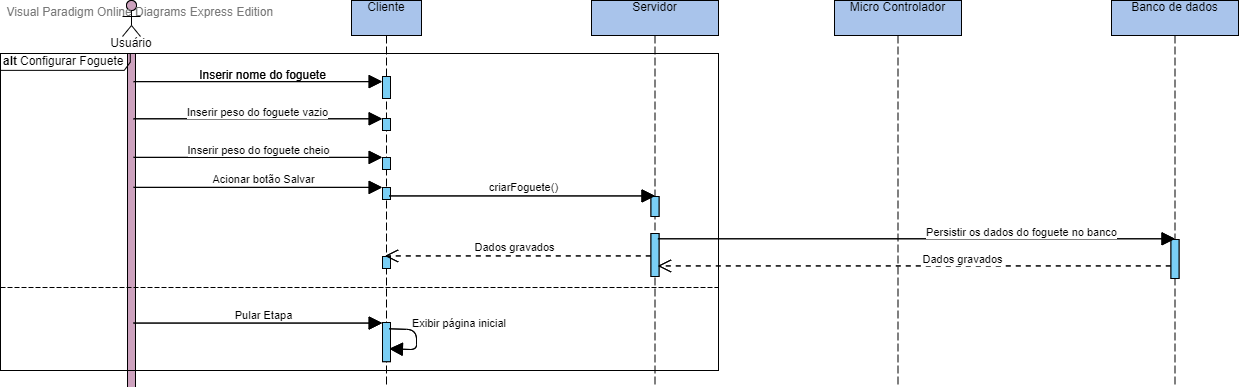
\includegraphics[width=1\textwidth, angle=0]{figuras/diagrama_sequencia_cadastro_foguete.png}
    \caption{Diagrama de sequencia representando o cadastro de foguetes. Fonte: Autor}
    \label{fig:Diagrama_sequencia_cadastr_foguete}
\end{figure}

\begin{figure}[htb]
    \centering
    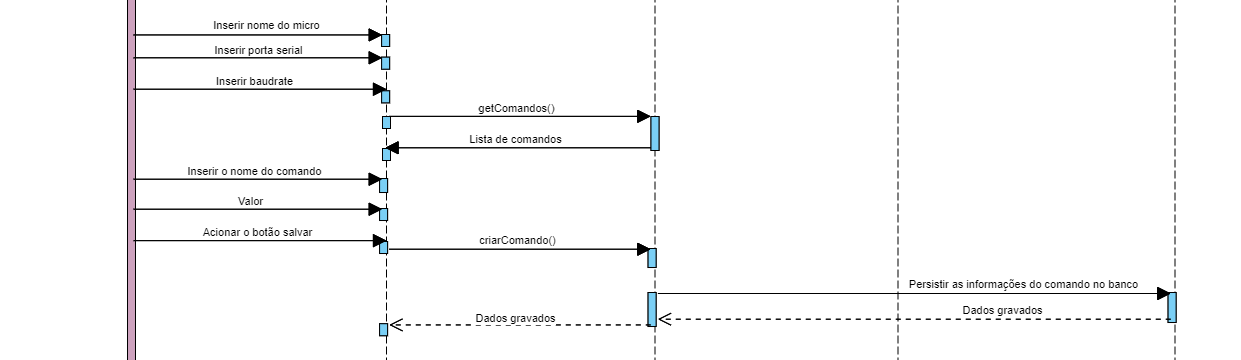
\includegraphics[width=1\textwidth, angle=0]{figuras/diagrama_sequencia_cadastro_micro.png}
    \caption{Diagrama de sequencia representando o cadastro de micro. Fonte: Autor}
    \label{fig:Diagrama_sequencia_cadastro_micro}
\end{figure}

\begin{figure}[htb]
    \centering
    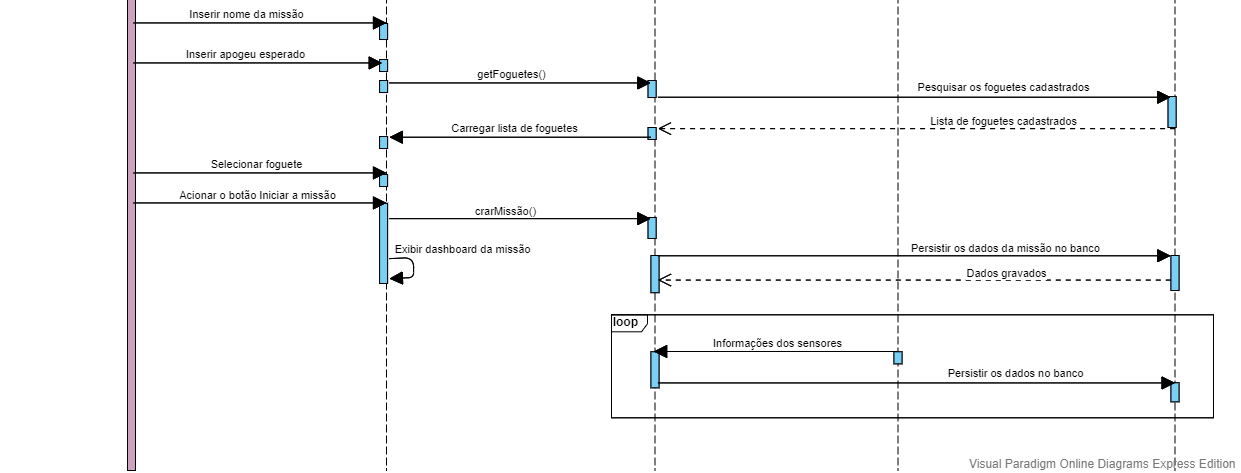
\includegraphics[width=1\textwidth, angle=0]{figuras/diagrama_sequencia_missao.png}
    \caption{Diagrama de sequencia representando o processo da missão. Fonte: Autor}
    \label{fig:Diagrama_sequencia_missao}
\end{figure}

\begin{figure}[htb]
    \centering
    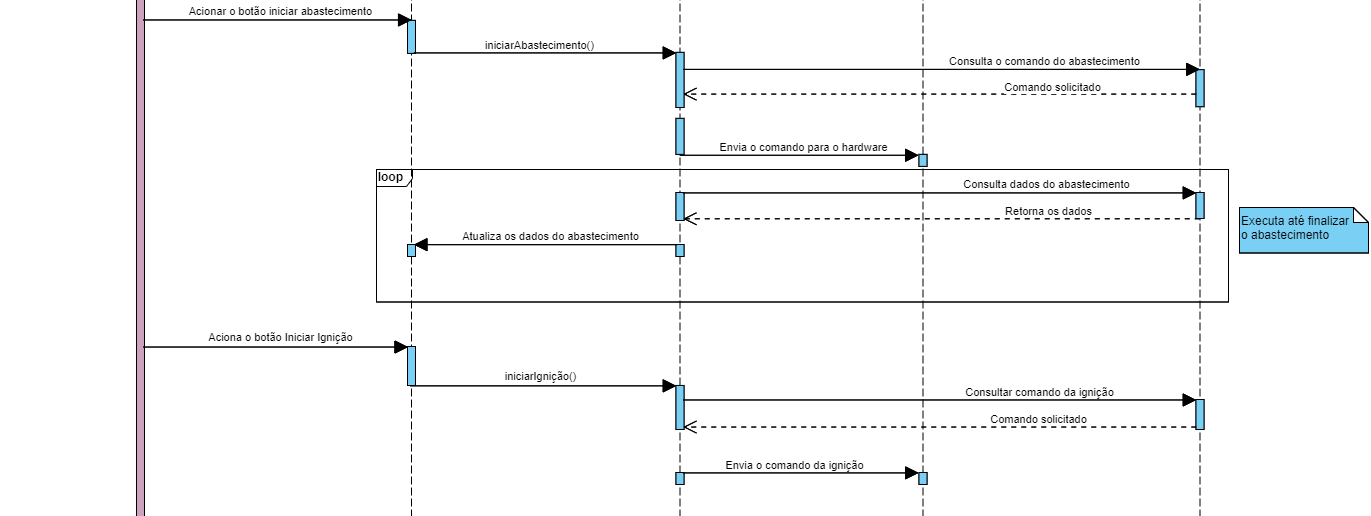
\includegraphics[width=1\textwidth, angle=0]{figuras/diagrama_sequencia_abastecimento.png}
    \caption{Diagrama de sequencia representando o processo de abastecimento. Fonte: Autor}
    \label{fig:Diagrama_sequencia_abastecimento}
\end{figure}

\begin{figure}[htb]
    \centering
    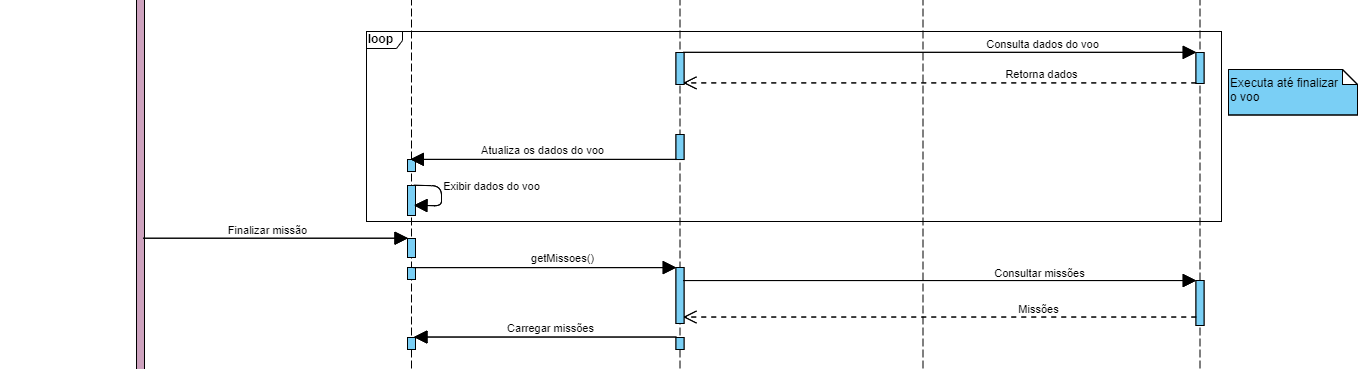
\includegraphics[width=1\textwidth, angle=0]{figuras/diagrama_sequencia_finaliza_missao.png}
    \caption{Diagrama de sequencia representando o processo de finalizar a missão. Fonte: Autor}
    \label{fig:Diagrama_sequencia_finaliza_missao}
\end{figure}

\begin{figure}[htb]
    \centering
    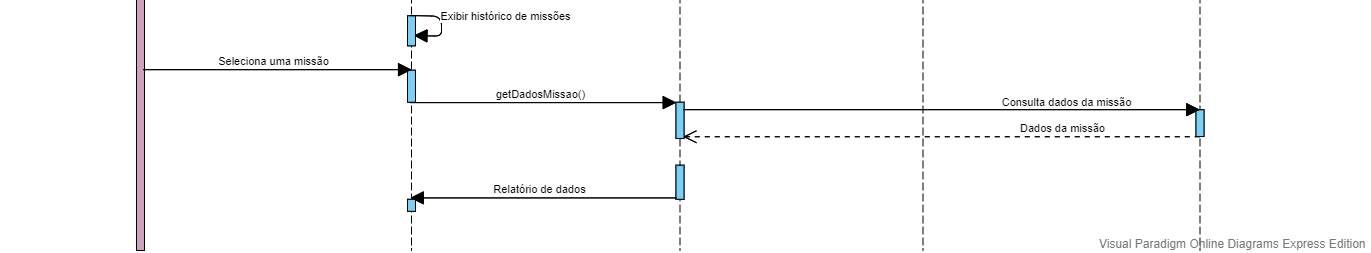
\includegraphics[width=1\textwidth, angle=0]{figuras/diagrama_sequencia_historico.png}
    \caption{Diagrama de sequencia representando o processo de histórico. Fonte: Autor}
    \label{fig:Diagrama_sequencia_historico}
\end{figure}





\chapter{Diagrama de blocos do sistema Versão Inicial}
\label{Diagrama de blocos do sistema}
\begin{figure}[htb]
    \centering
    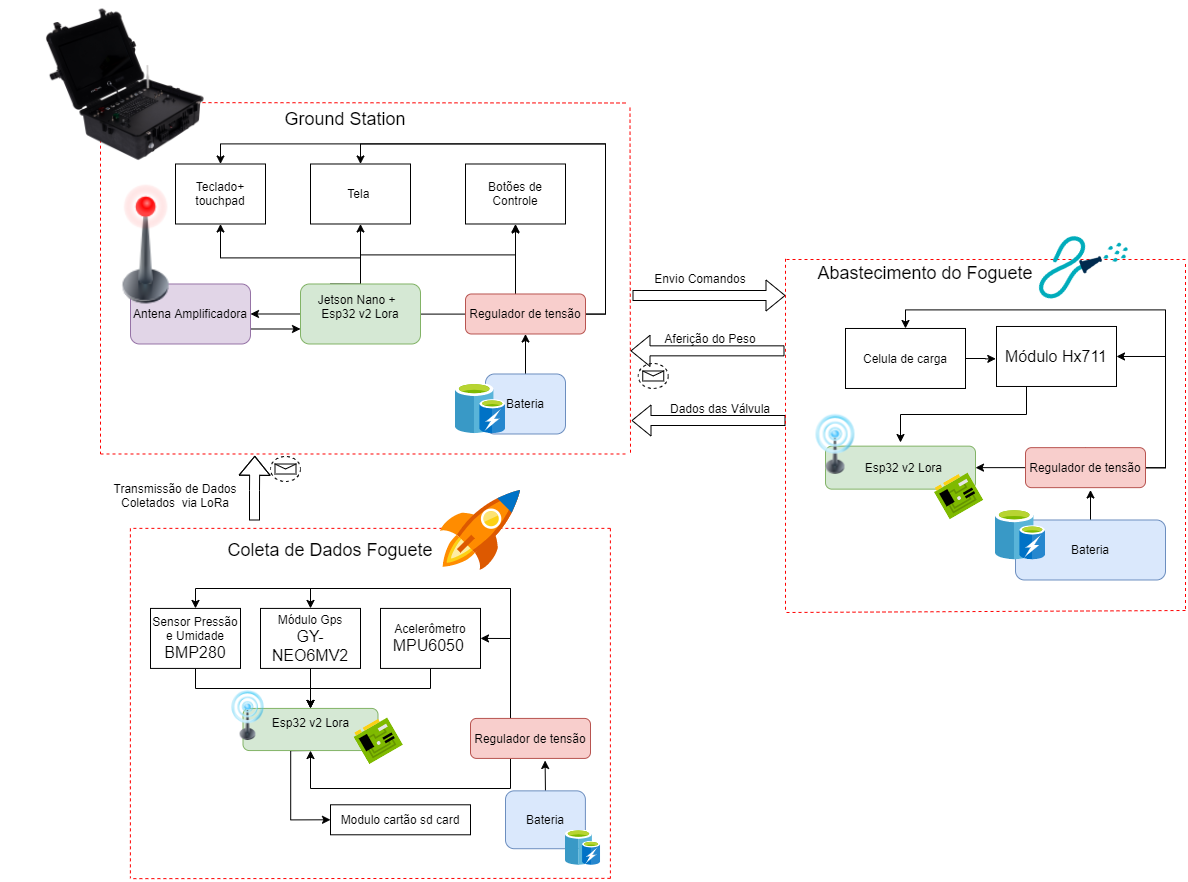
\includegraphics[width=1\textwidth, angle=90]{figuras/diagrama pi2 (2).png}
    \caption{Diagrama de blocos do projeto. Fonte: Autor}
    \label{fig:Diagrama de Blocos}
\end{figure}

%\chapter{Diagrama de Blocos/Comunicação}
%\label{Diagrama_Geral}
%\begin{figure}[htb]
 %   \centering
 %   \includegraphics[width=1.1\textwidth, angle=90]{figuras/Diagrama_Geral.png}
  %  \caption{Diagrama de comunicação do projeto. Fonte: Autor}
  %  \url{https://drive.google.com/file/d/12-pXv5L2Z5AuyWWVIr8VZ4WMghu7SYDw/view?usp=sharing}
  %  \label{fig:Diagrama_Geral}
%\end{figure}

\chapter{Diagramas elétricos}
\label{diag_eletrico}

\begin{figure}[H]
    \centering
    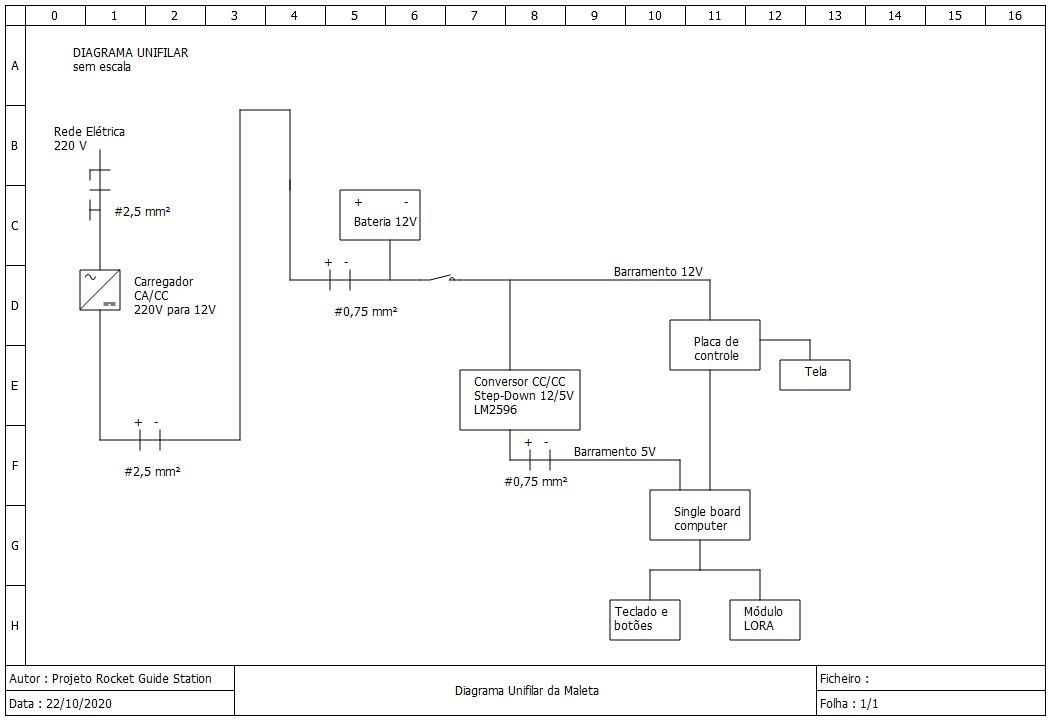
\includegraphics[width=1.0\textwidth, angle=270]{figuras/diamalgcs.jpeg}
    \caption{Diagrama unifilar GCS}
    \label{fig:diagrama_unifilar_01}
\end{figure}

\begin{figure}[H]
    \centering
    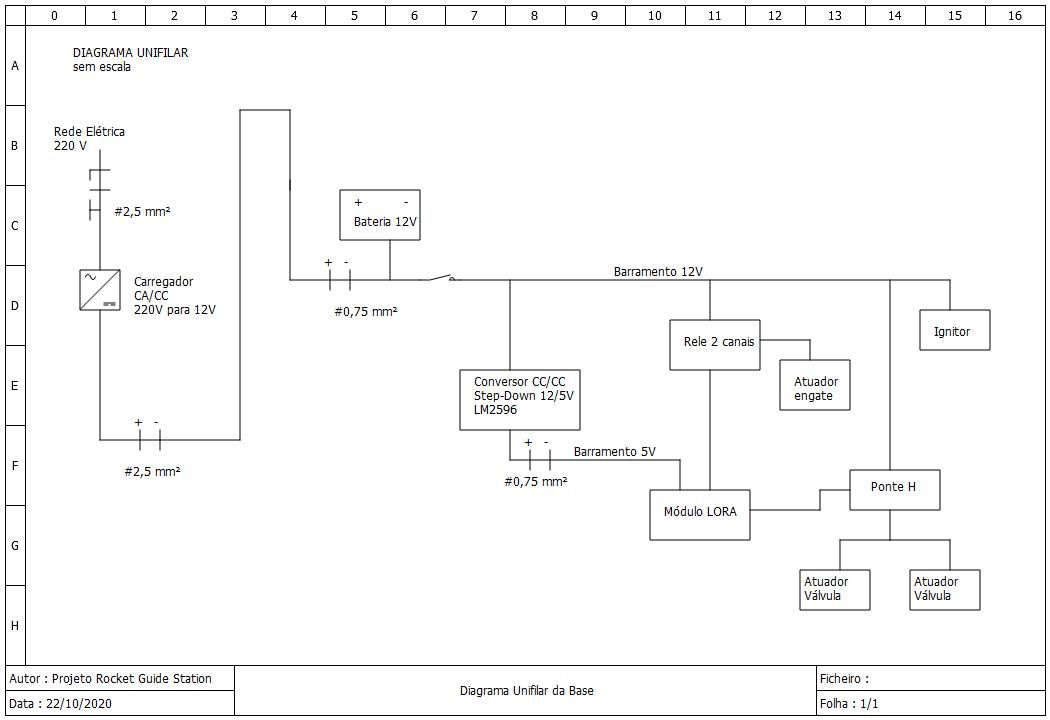
\includegraphics[width=1.0\textwidth, angle=270]{figuras/diamalsup.jpeg}
    \caption{Diagrama unifilar abastecimento}
    \label{fig:diagrama_unifilar_02}
\end{figure}

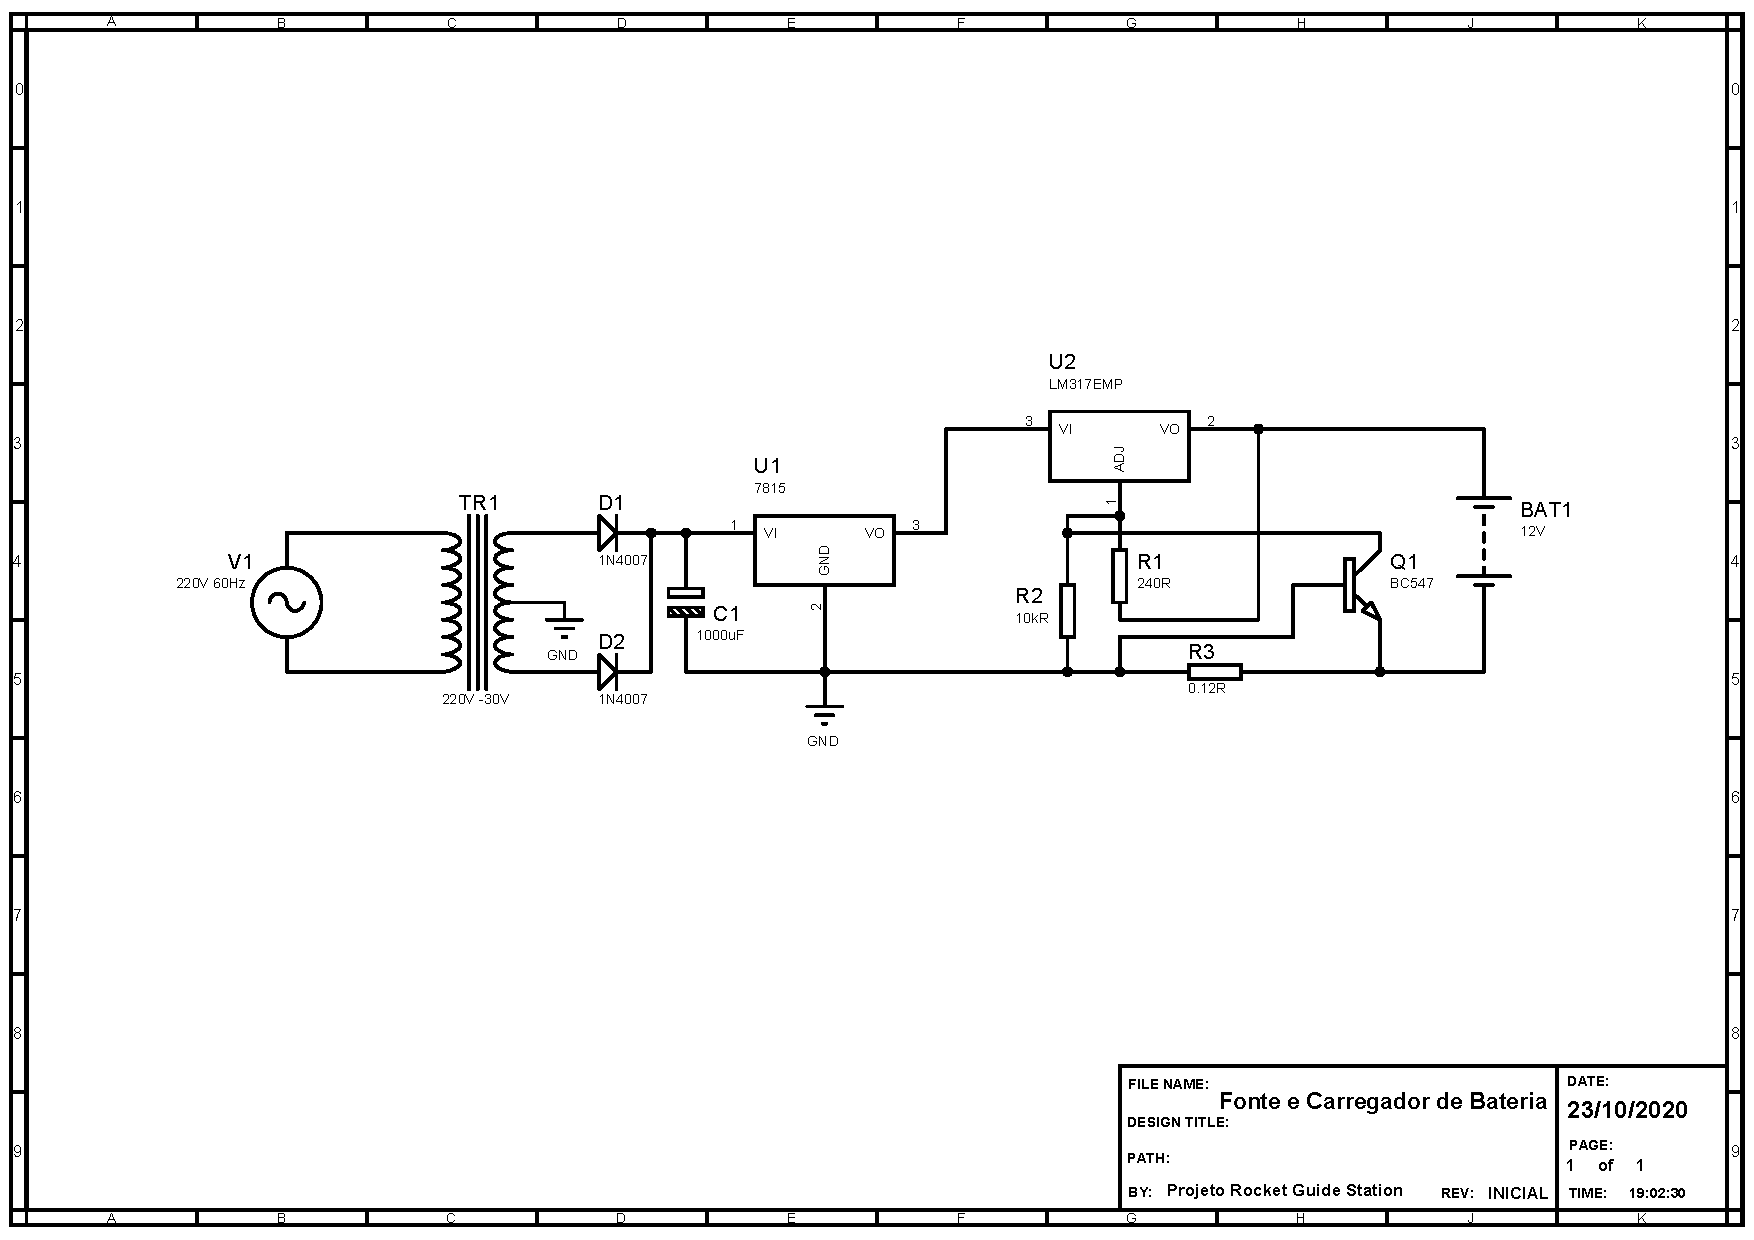
\includepdf[pages=-, angle=270]{figuras/circuitoeletrico.pdf}



\chapter{Esboço inicial e CAD}
\label{CAD}

\begin{figure}[htb]
    \centering
    \includegraphics[width=0.5\textwidth , angle=90 ]{figuras/EsboçoInicial_V_1.jpg}
    \caption{Esboço inicial}
    \label{fig:esboço}
\end{figure}

\begin{figure} [H]
\centering
  \subfigure[aberto]{
    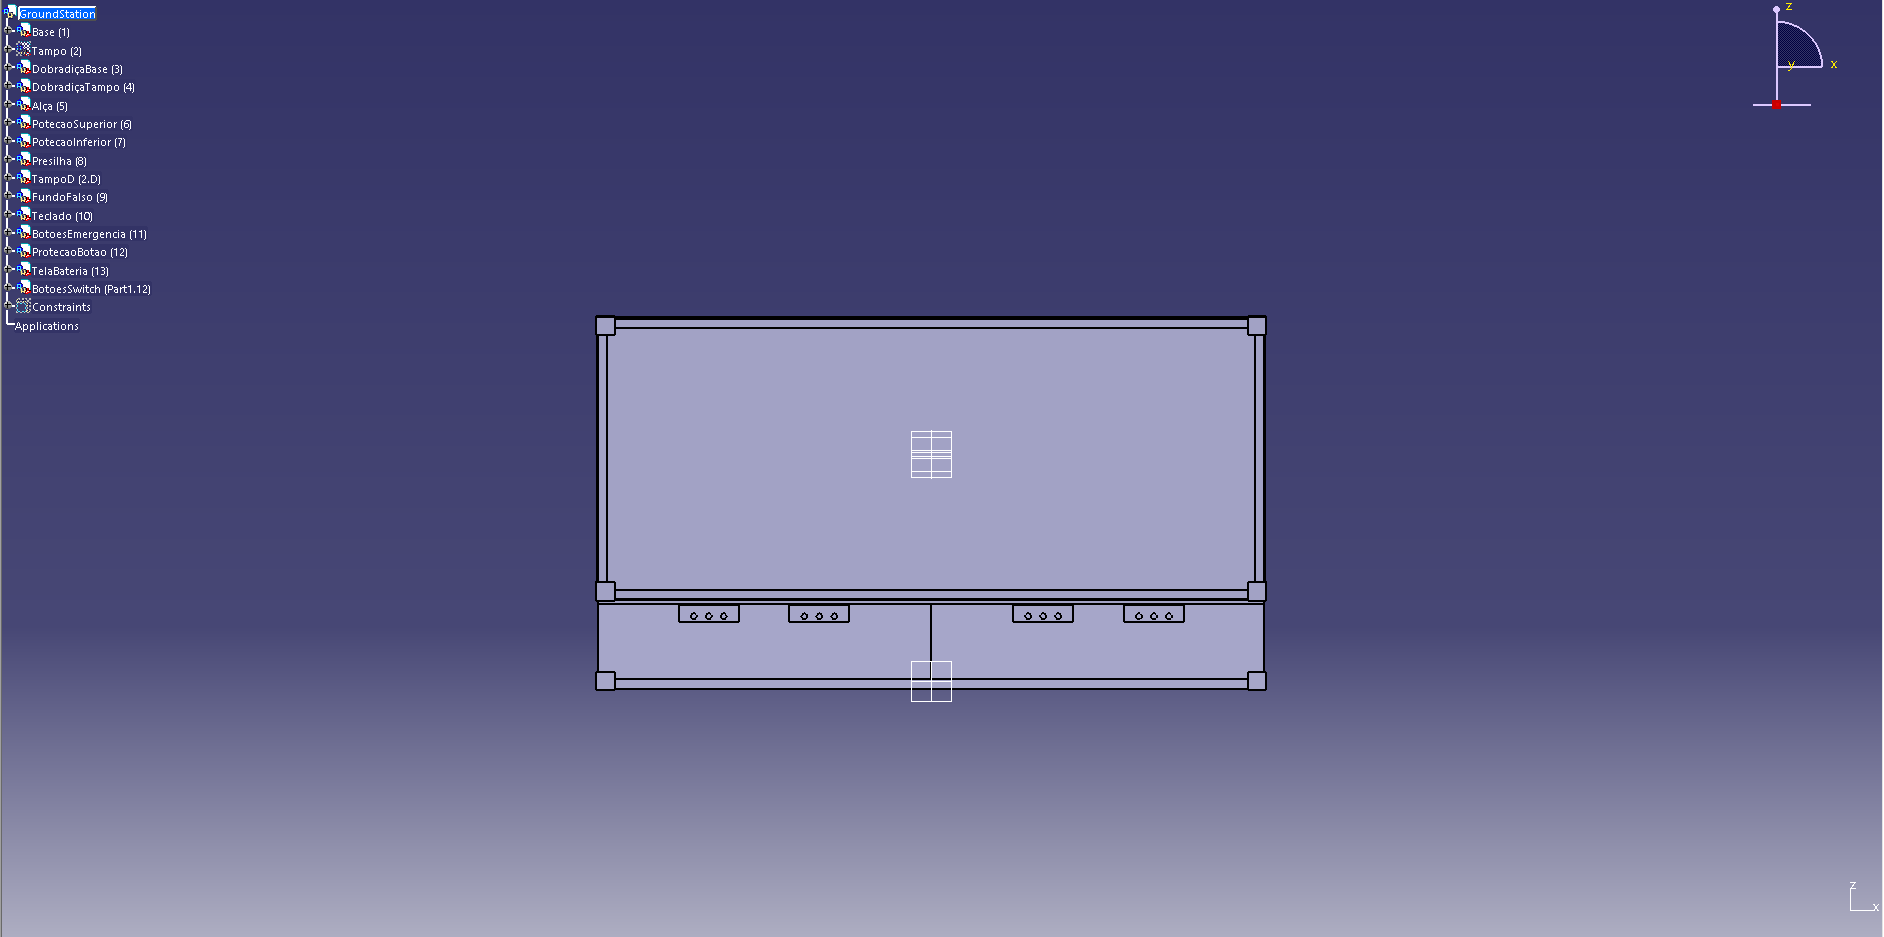
\includegraphics[width=7cm]{figuras/Back1.PNG}
  } 
  \subfigure[fechado]{ 
    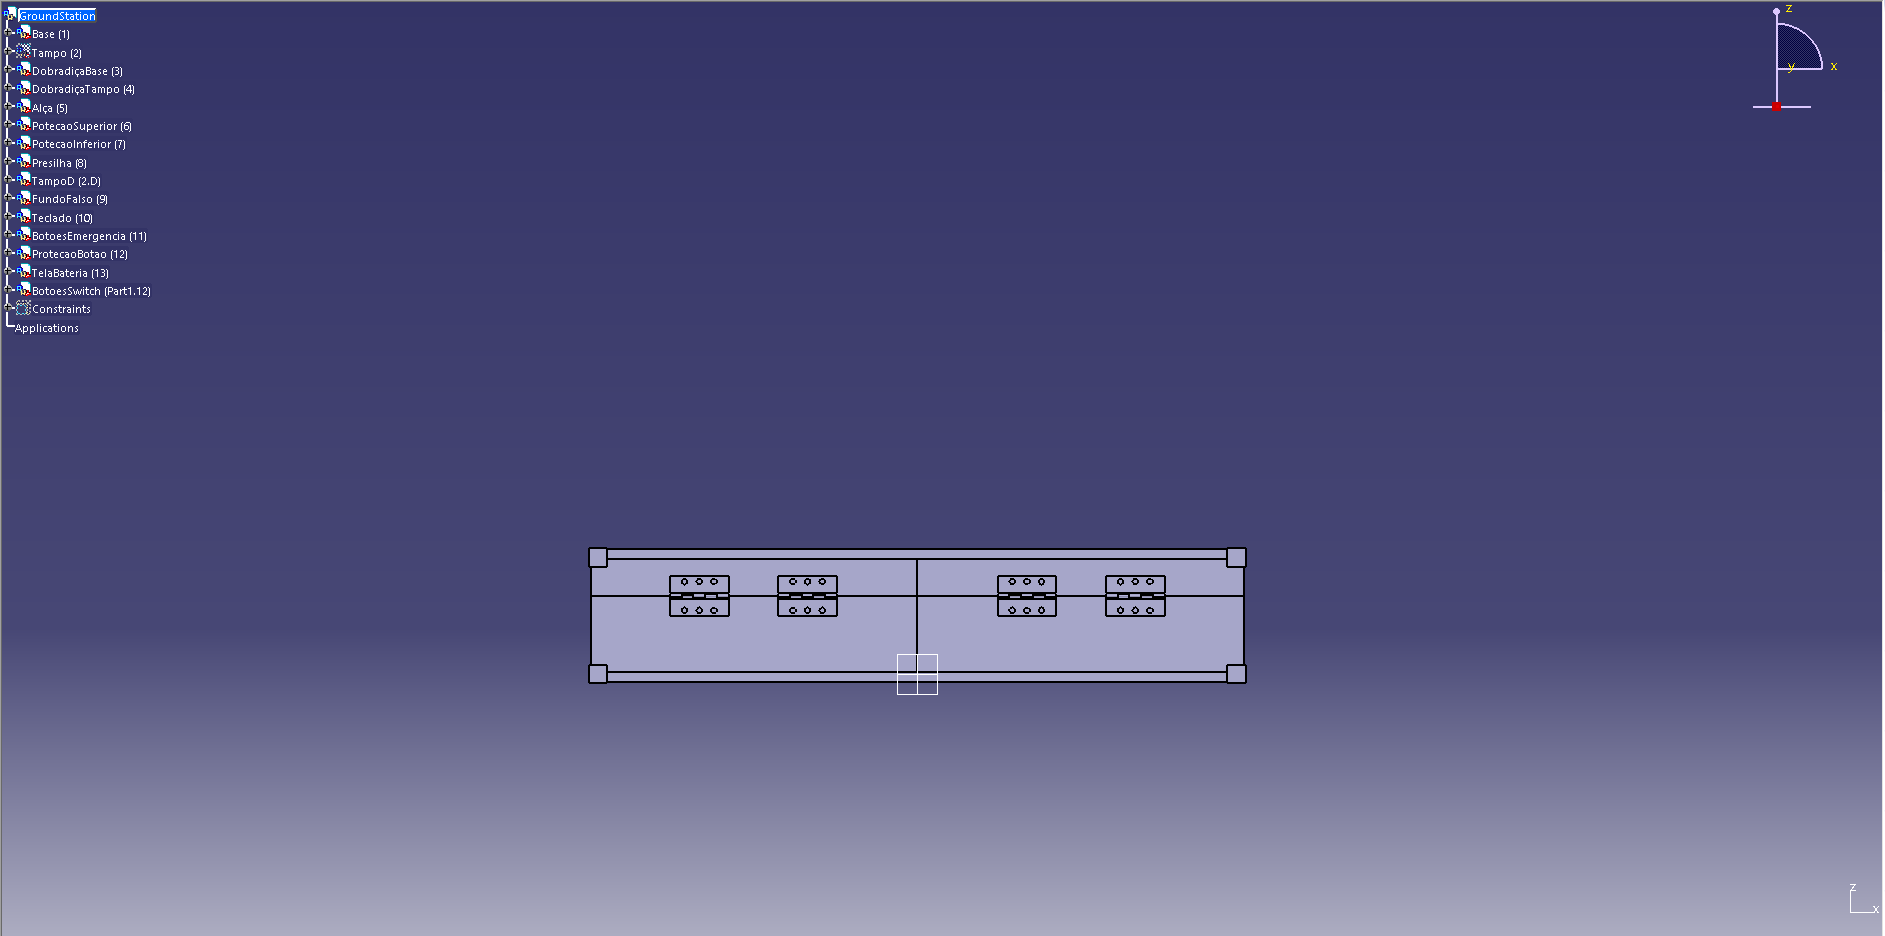
\includegraphics[width=7cm]{figuras/Back2.PNG}
  } 
  \caption{CAD da maleta verso}
\end{figure}

\begin{figure} [H]
\centering
  \subfigure[aberto]{
    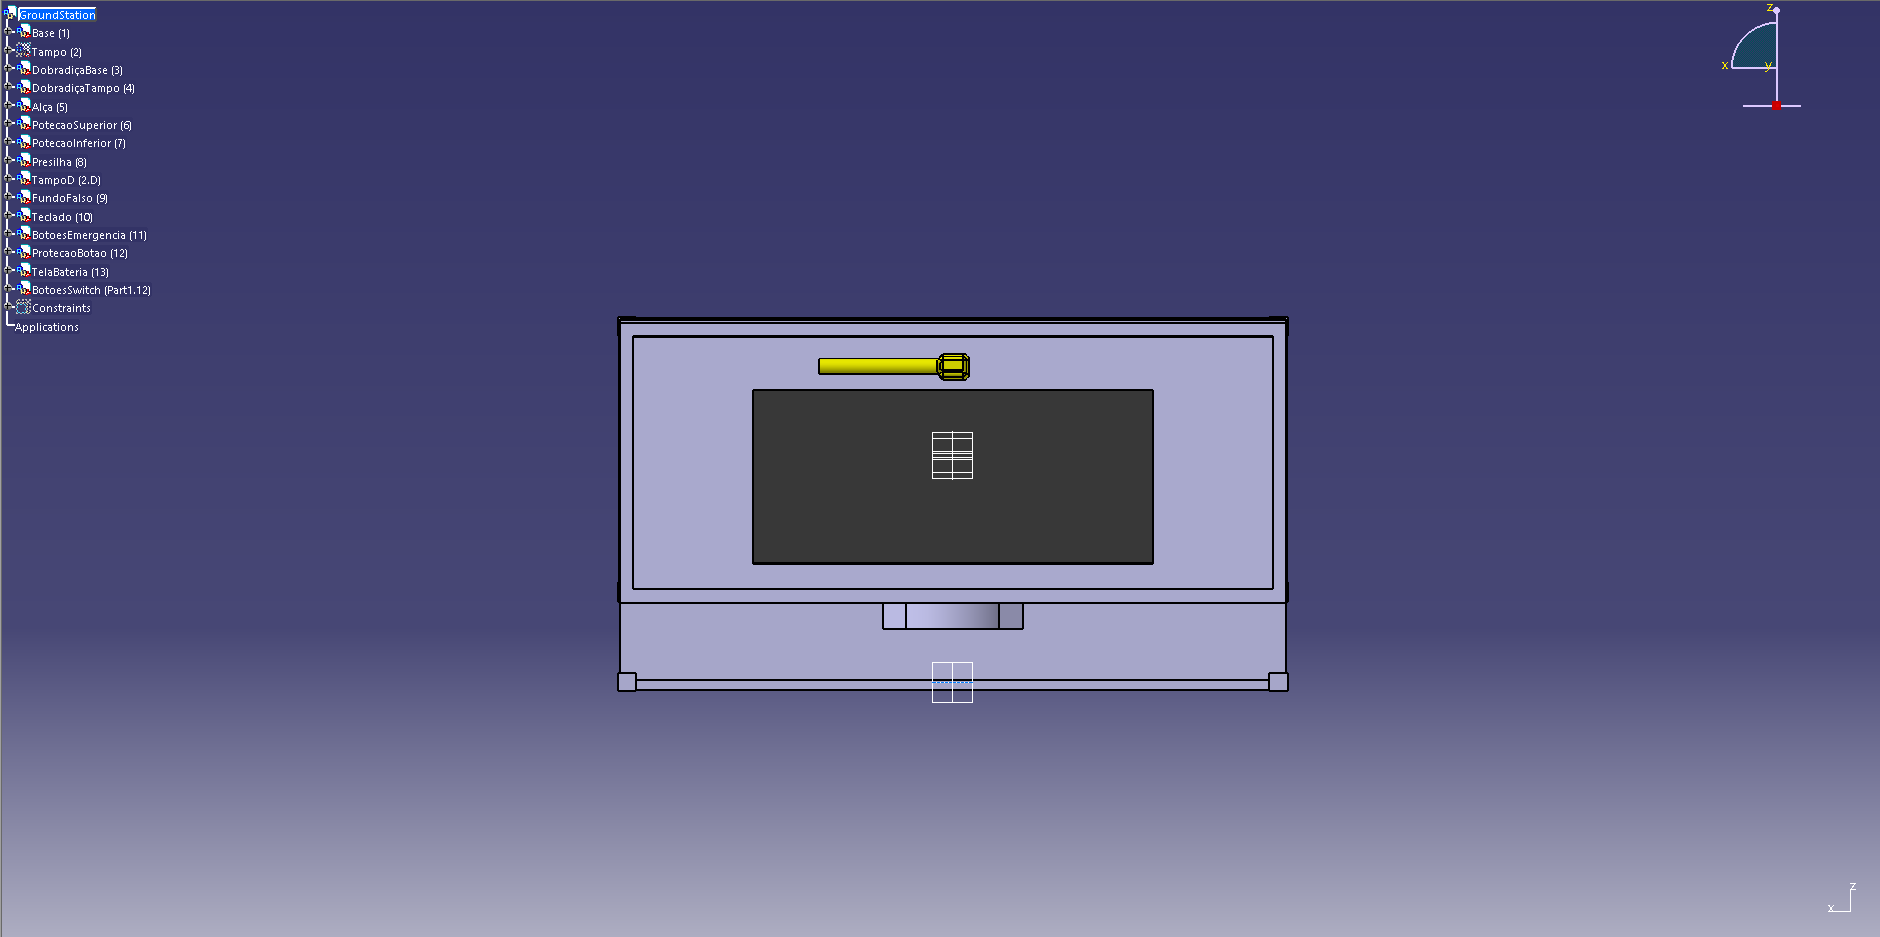
\includegraphics[width=7cm]{figuras/Front1.PNG}
  } 
  \subfigure[fechado]{ 
    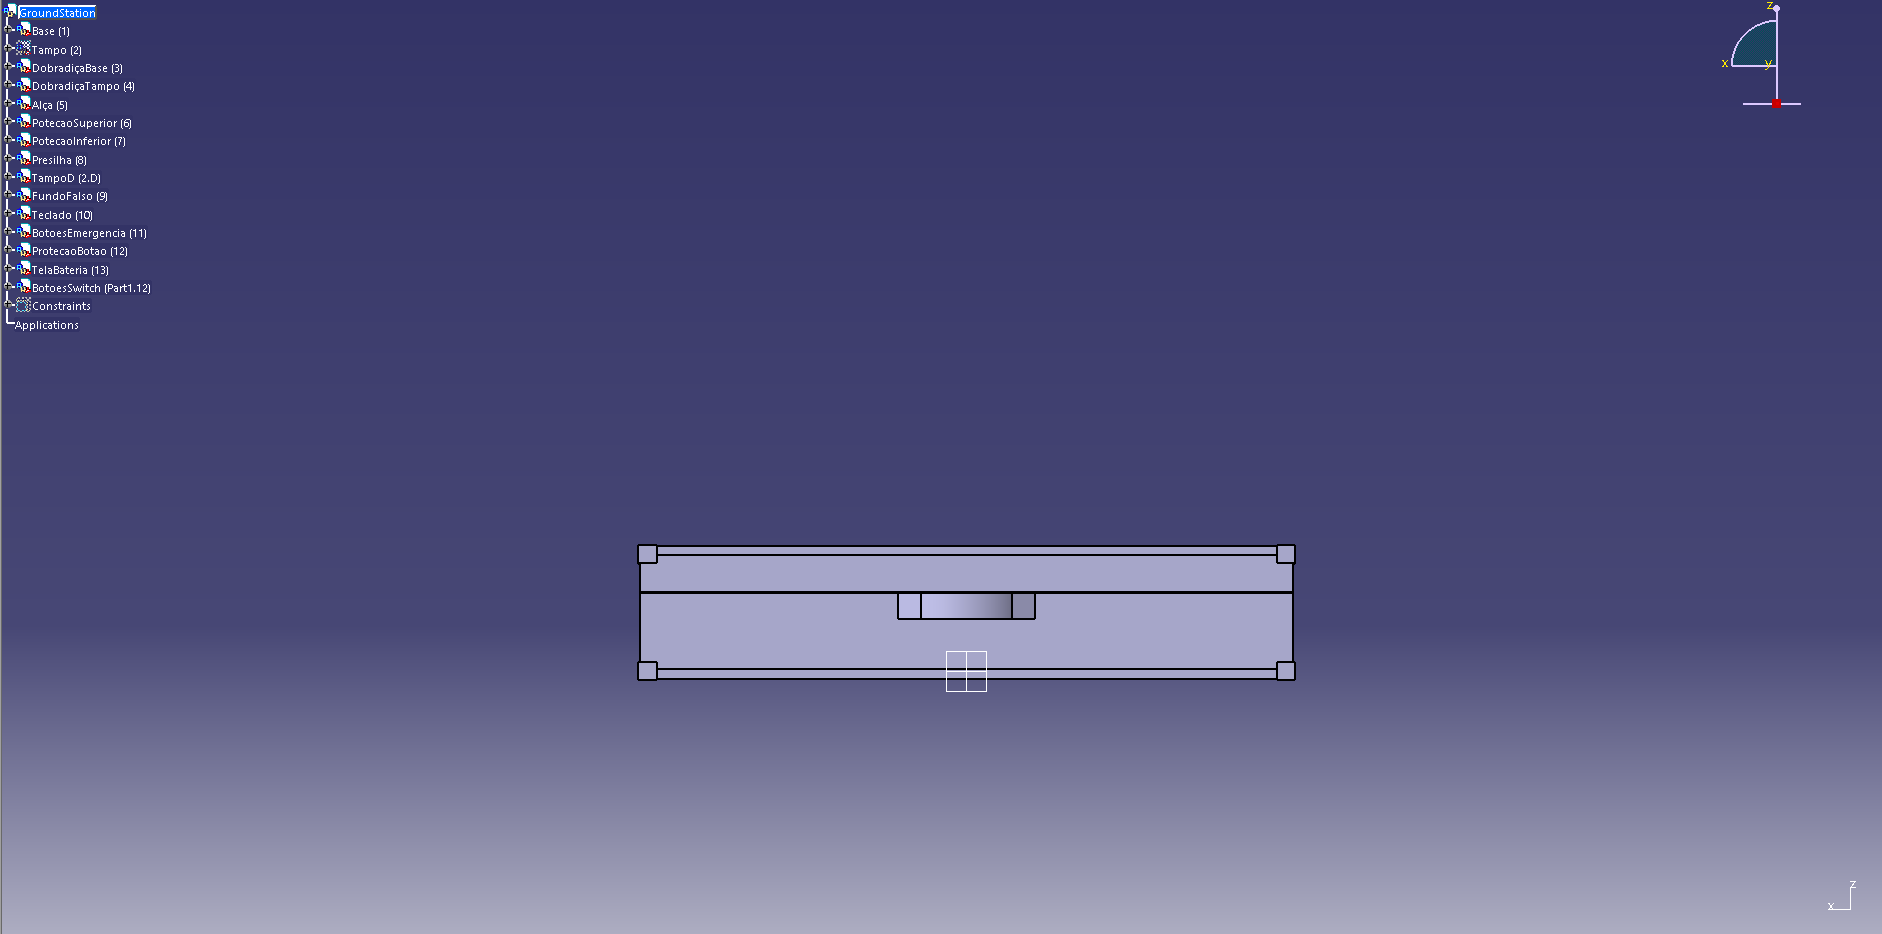
\includegraphics[width=7cm]{figuras/Front2.PNG}
  } 
  \caption{CAD's da maleta frente}
\end{figure}

\begin{figure} [H]
\centering
  \subfigure[aberto]{
    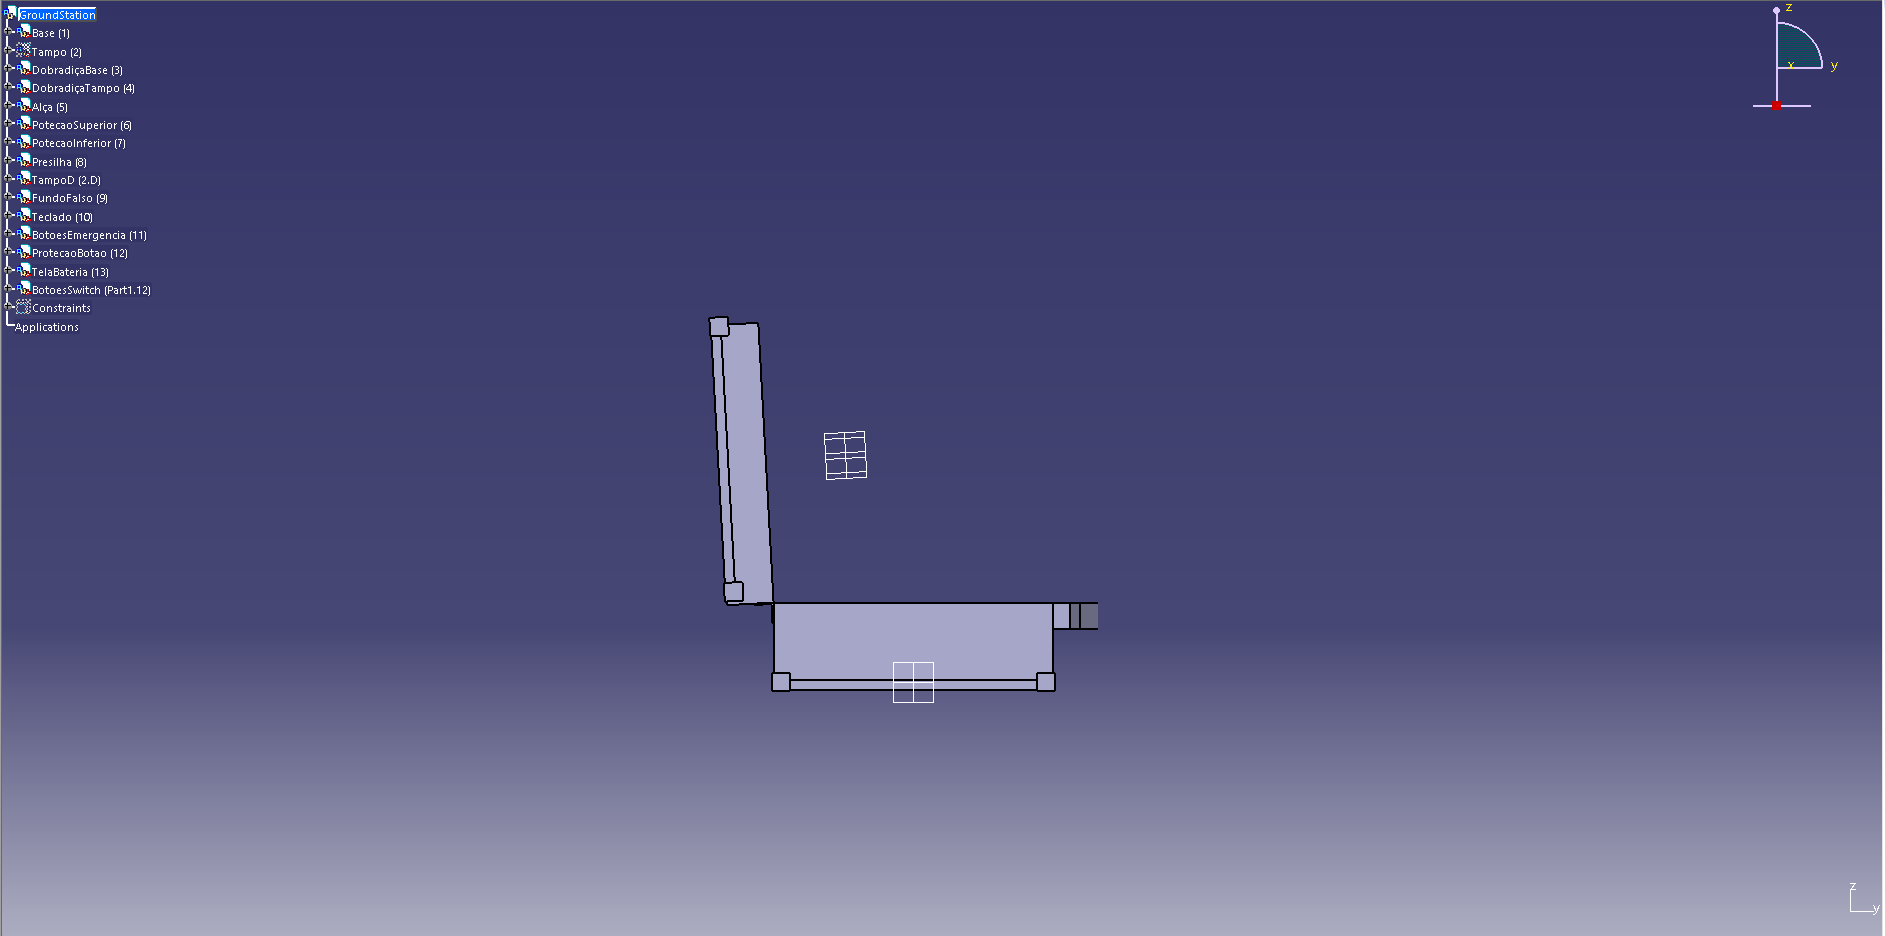
\includegraphics[width=7cm]{figuras/Lateral1.PNG}
  } 
  \subfigure[fechado]{ 
    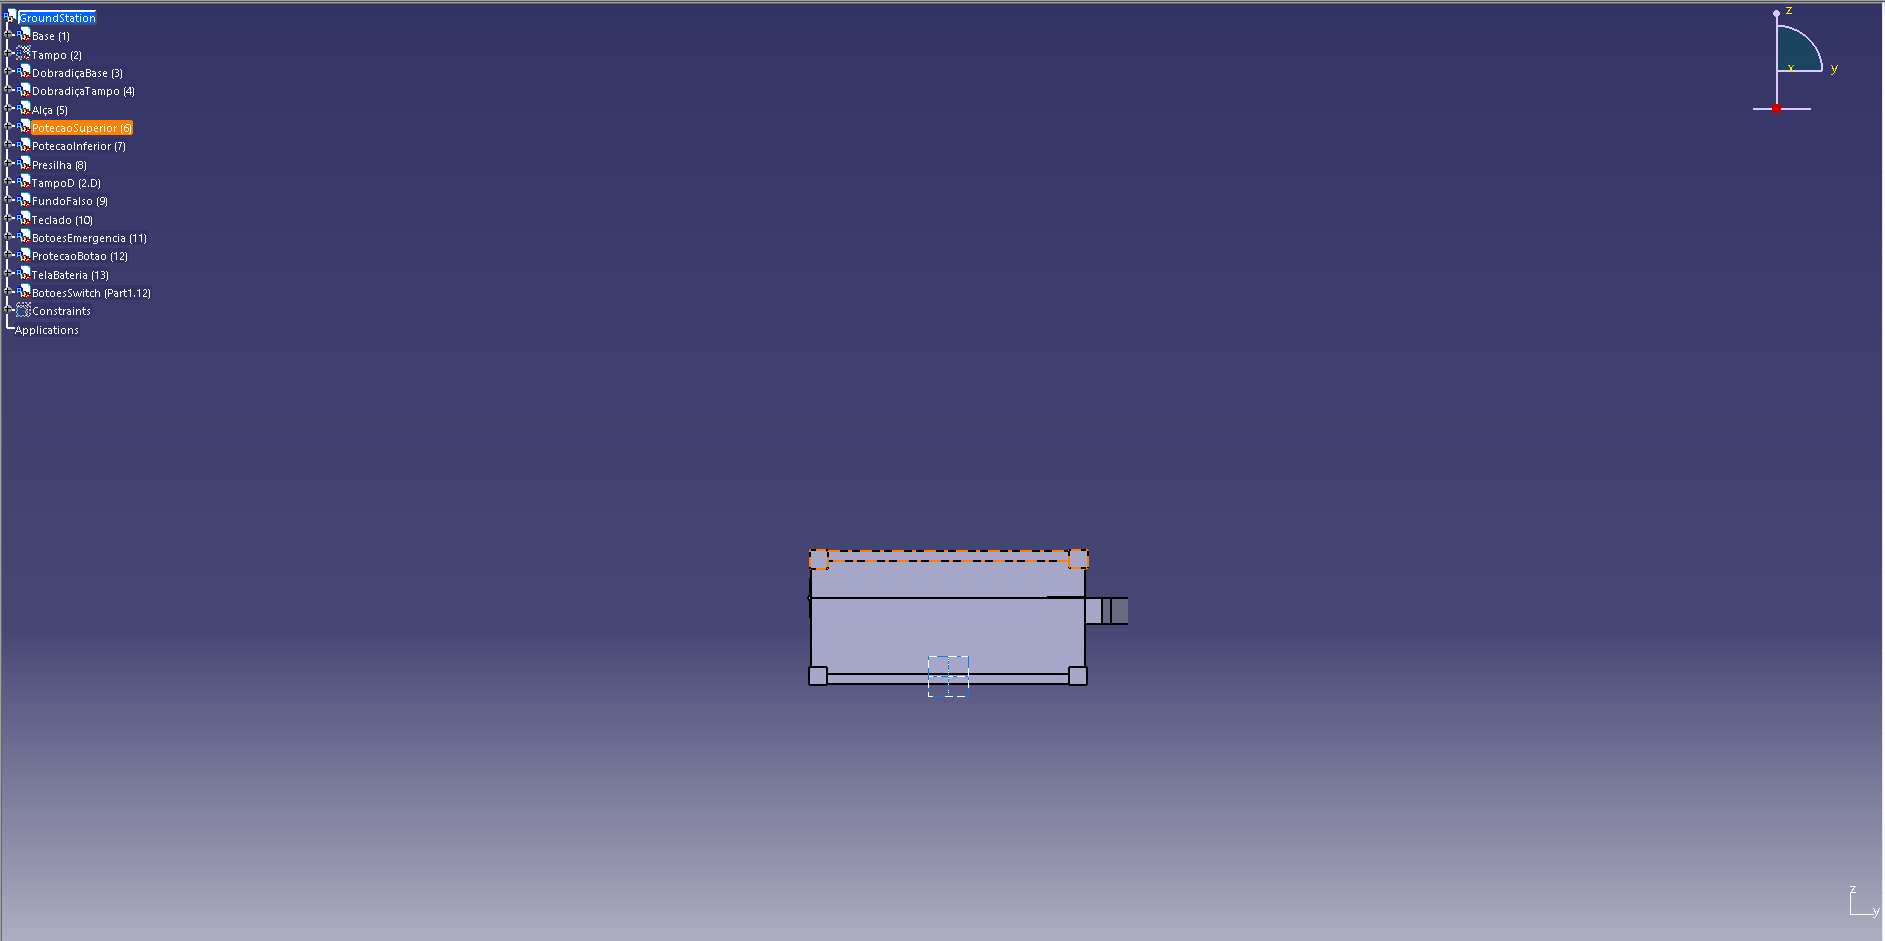
\includegraphics[width=7cm]{figuras/Lateral2.PNG}
  } 
  \caption{CAD's da maleta lateral}
\end{figure}

\begin{figure} [H]
\centering
  \subfigure[aberto]{
    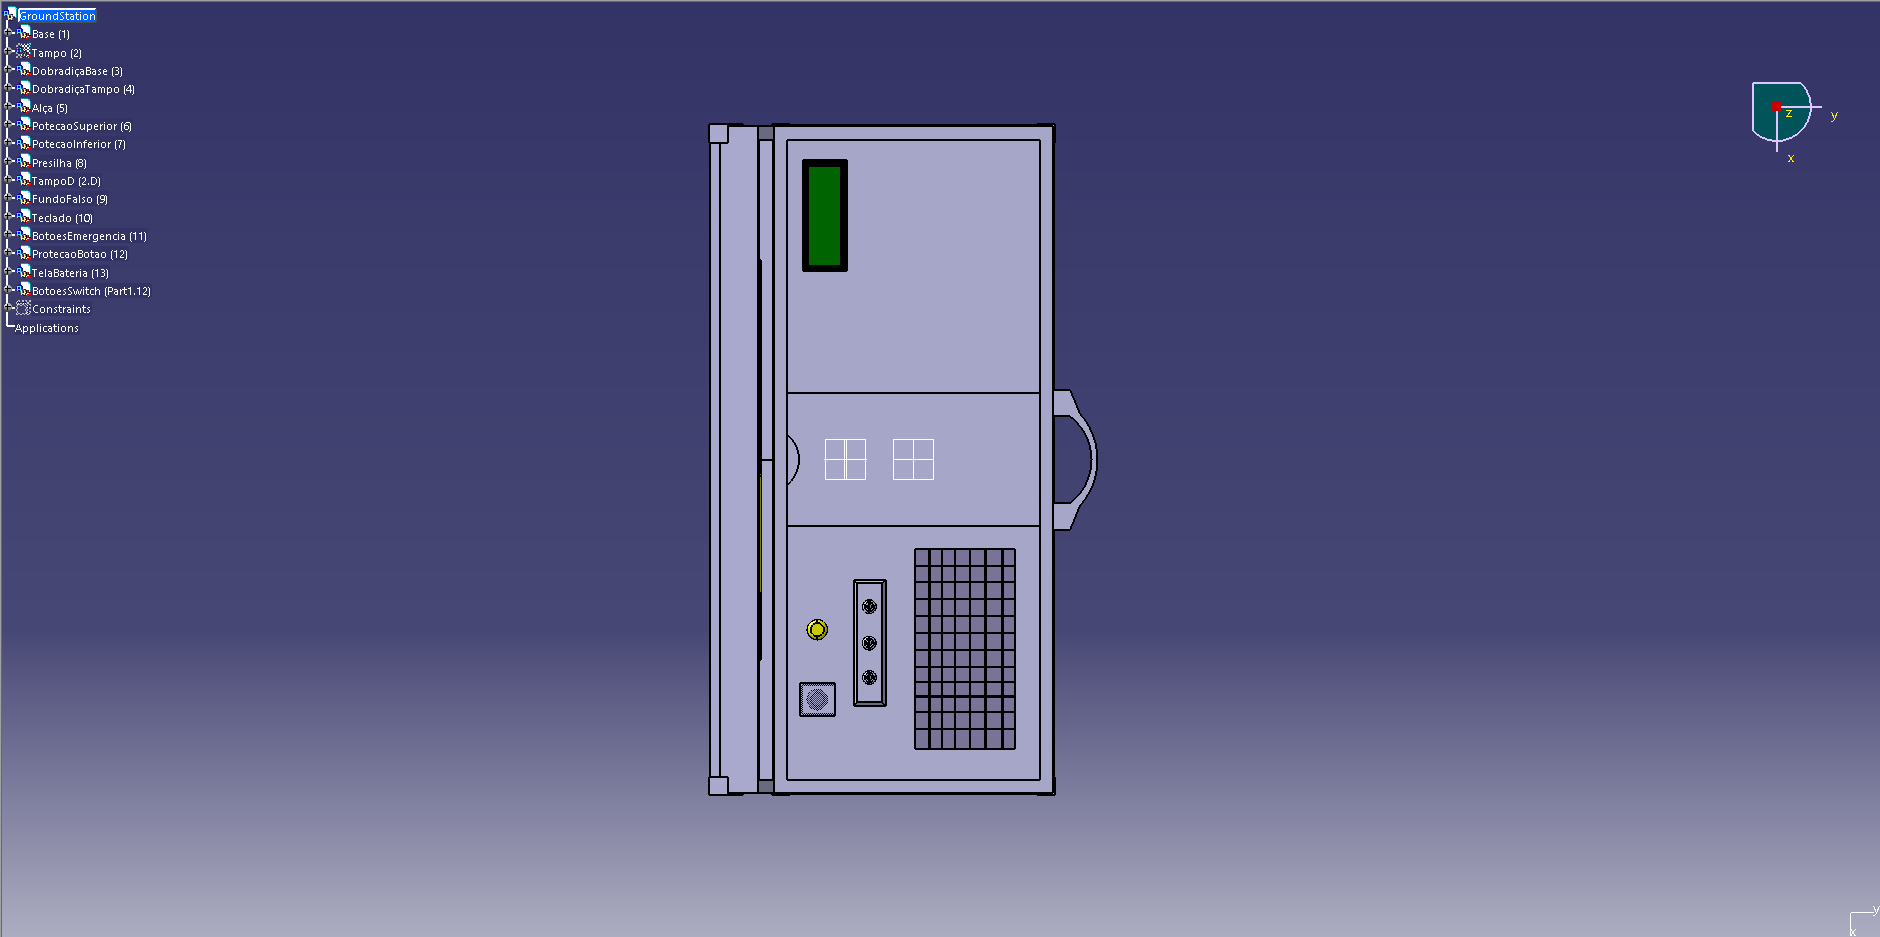
\includegraphics[width=7cm]{figuras/Sup1.PNG}
  } 
  \subfigure[fechado]{ 
    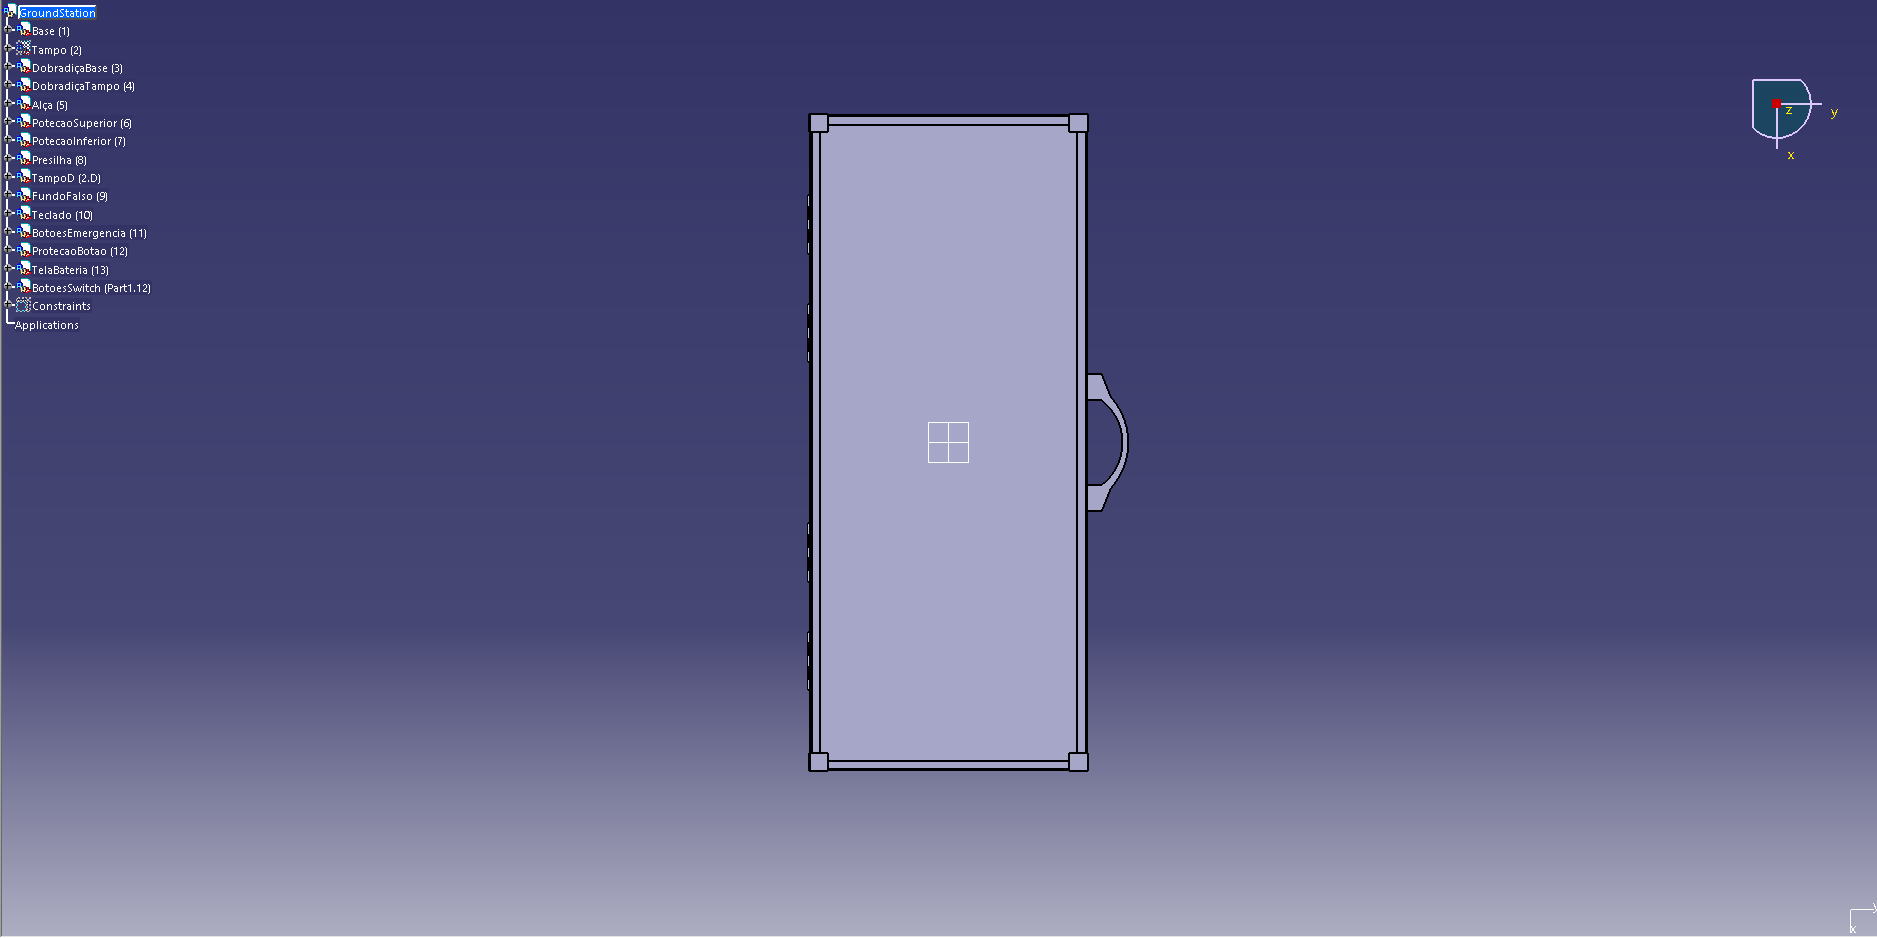
\includegraphics[width=7cm]{figuras/Sup2.PNG}
  } 
  \caption{CAD's da maleta superior}
\end{figure}

\begin{figure} [H]
\centering
  \subfigure[aberto]{
    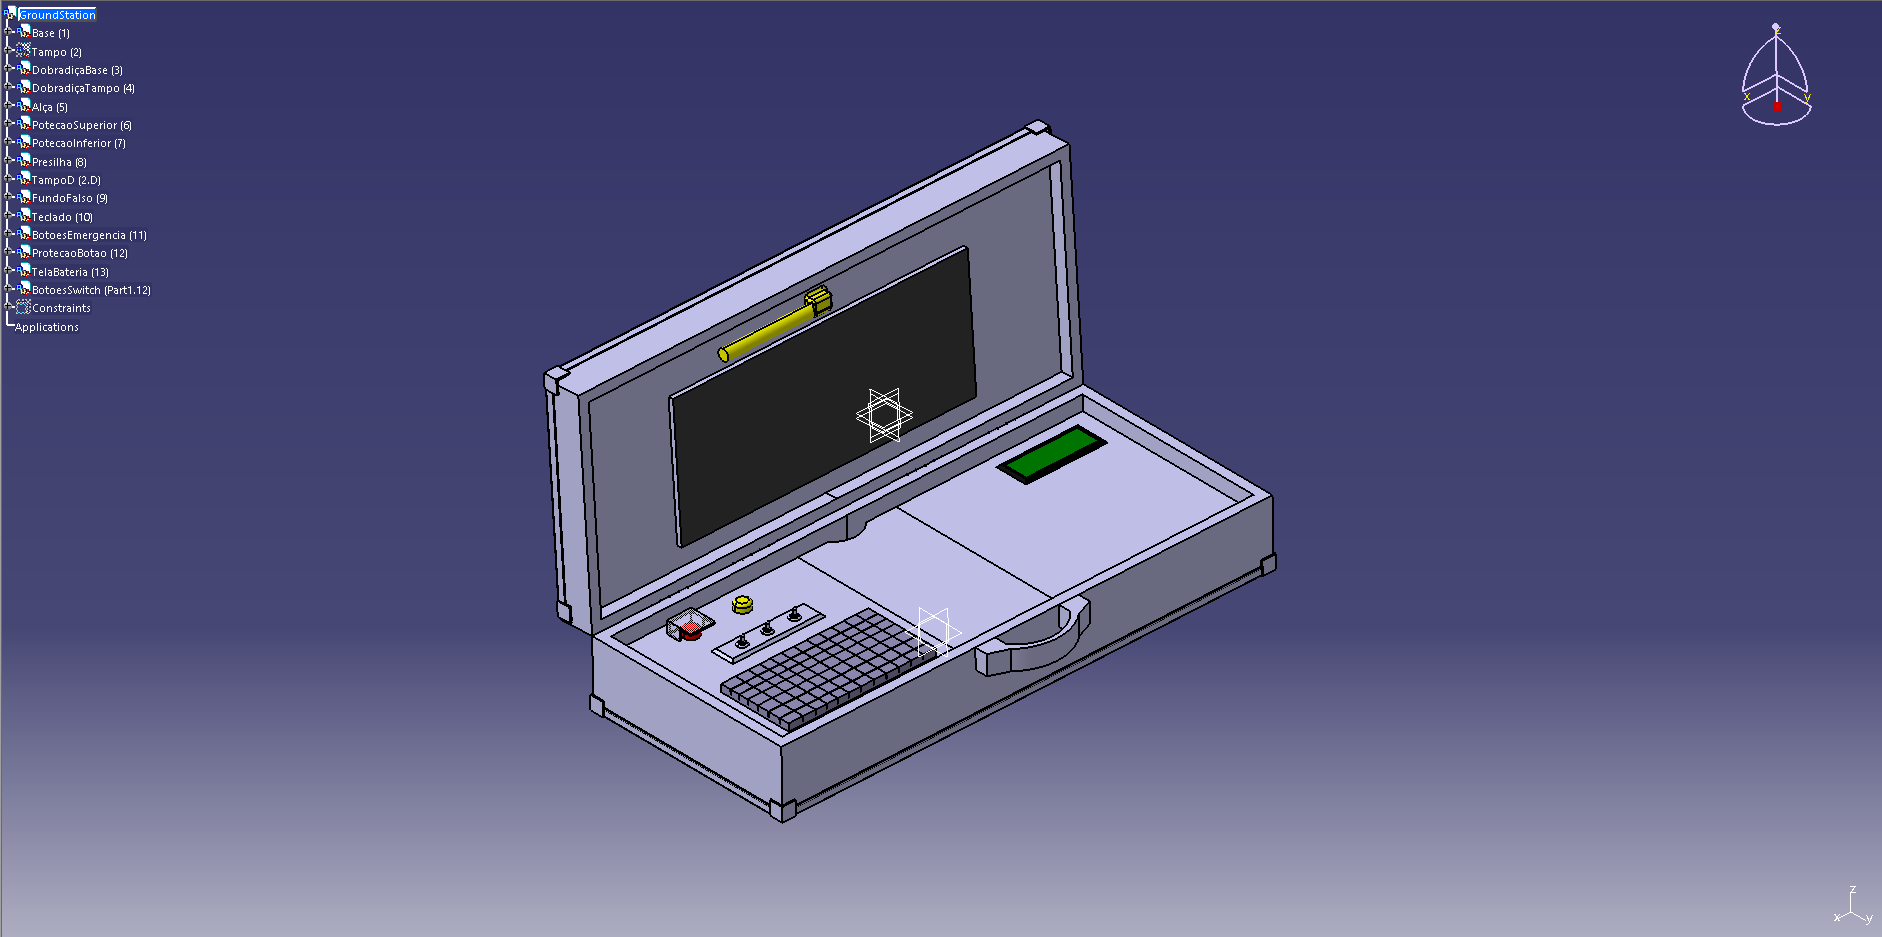
\includegraphics[width=7cm]{figuras/Iso1.PNG}
  } 
  \subfigure[fechada]{ 
    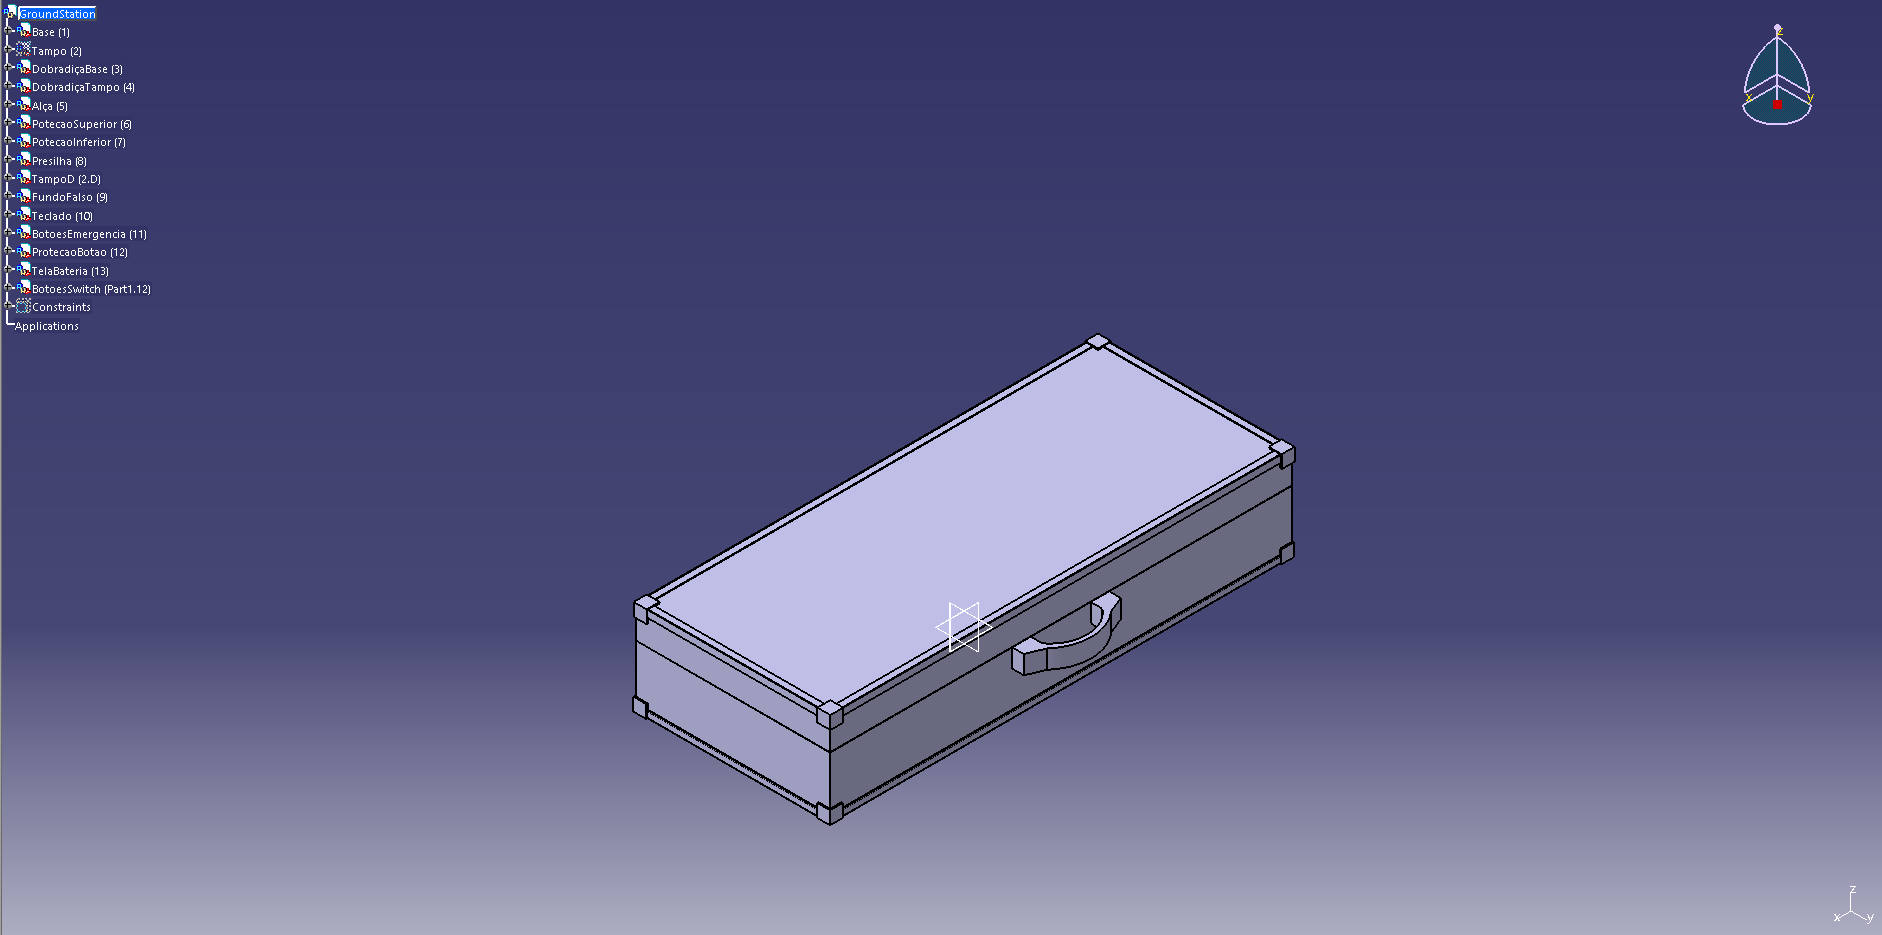
\includegraphics[width=7cm]{figuras/Iso2.PNG}
  } 
  \caption{CAD's da maleta isométrica}
\end{figure}


\chapter{Desenhos Técnicos}
\label{Drafts_do_projeto}

%\section{GCS}

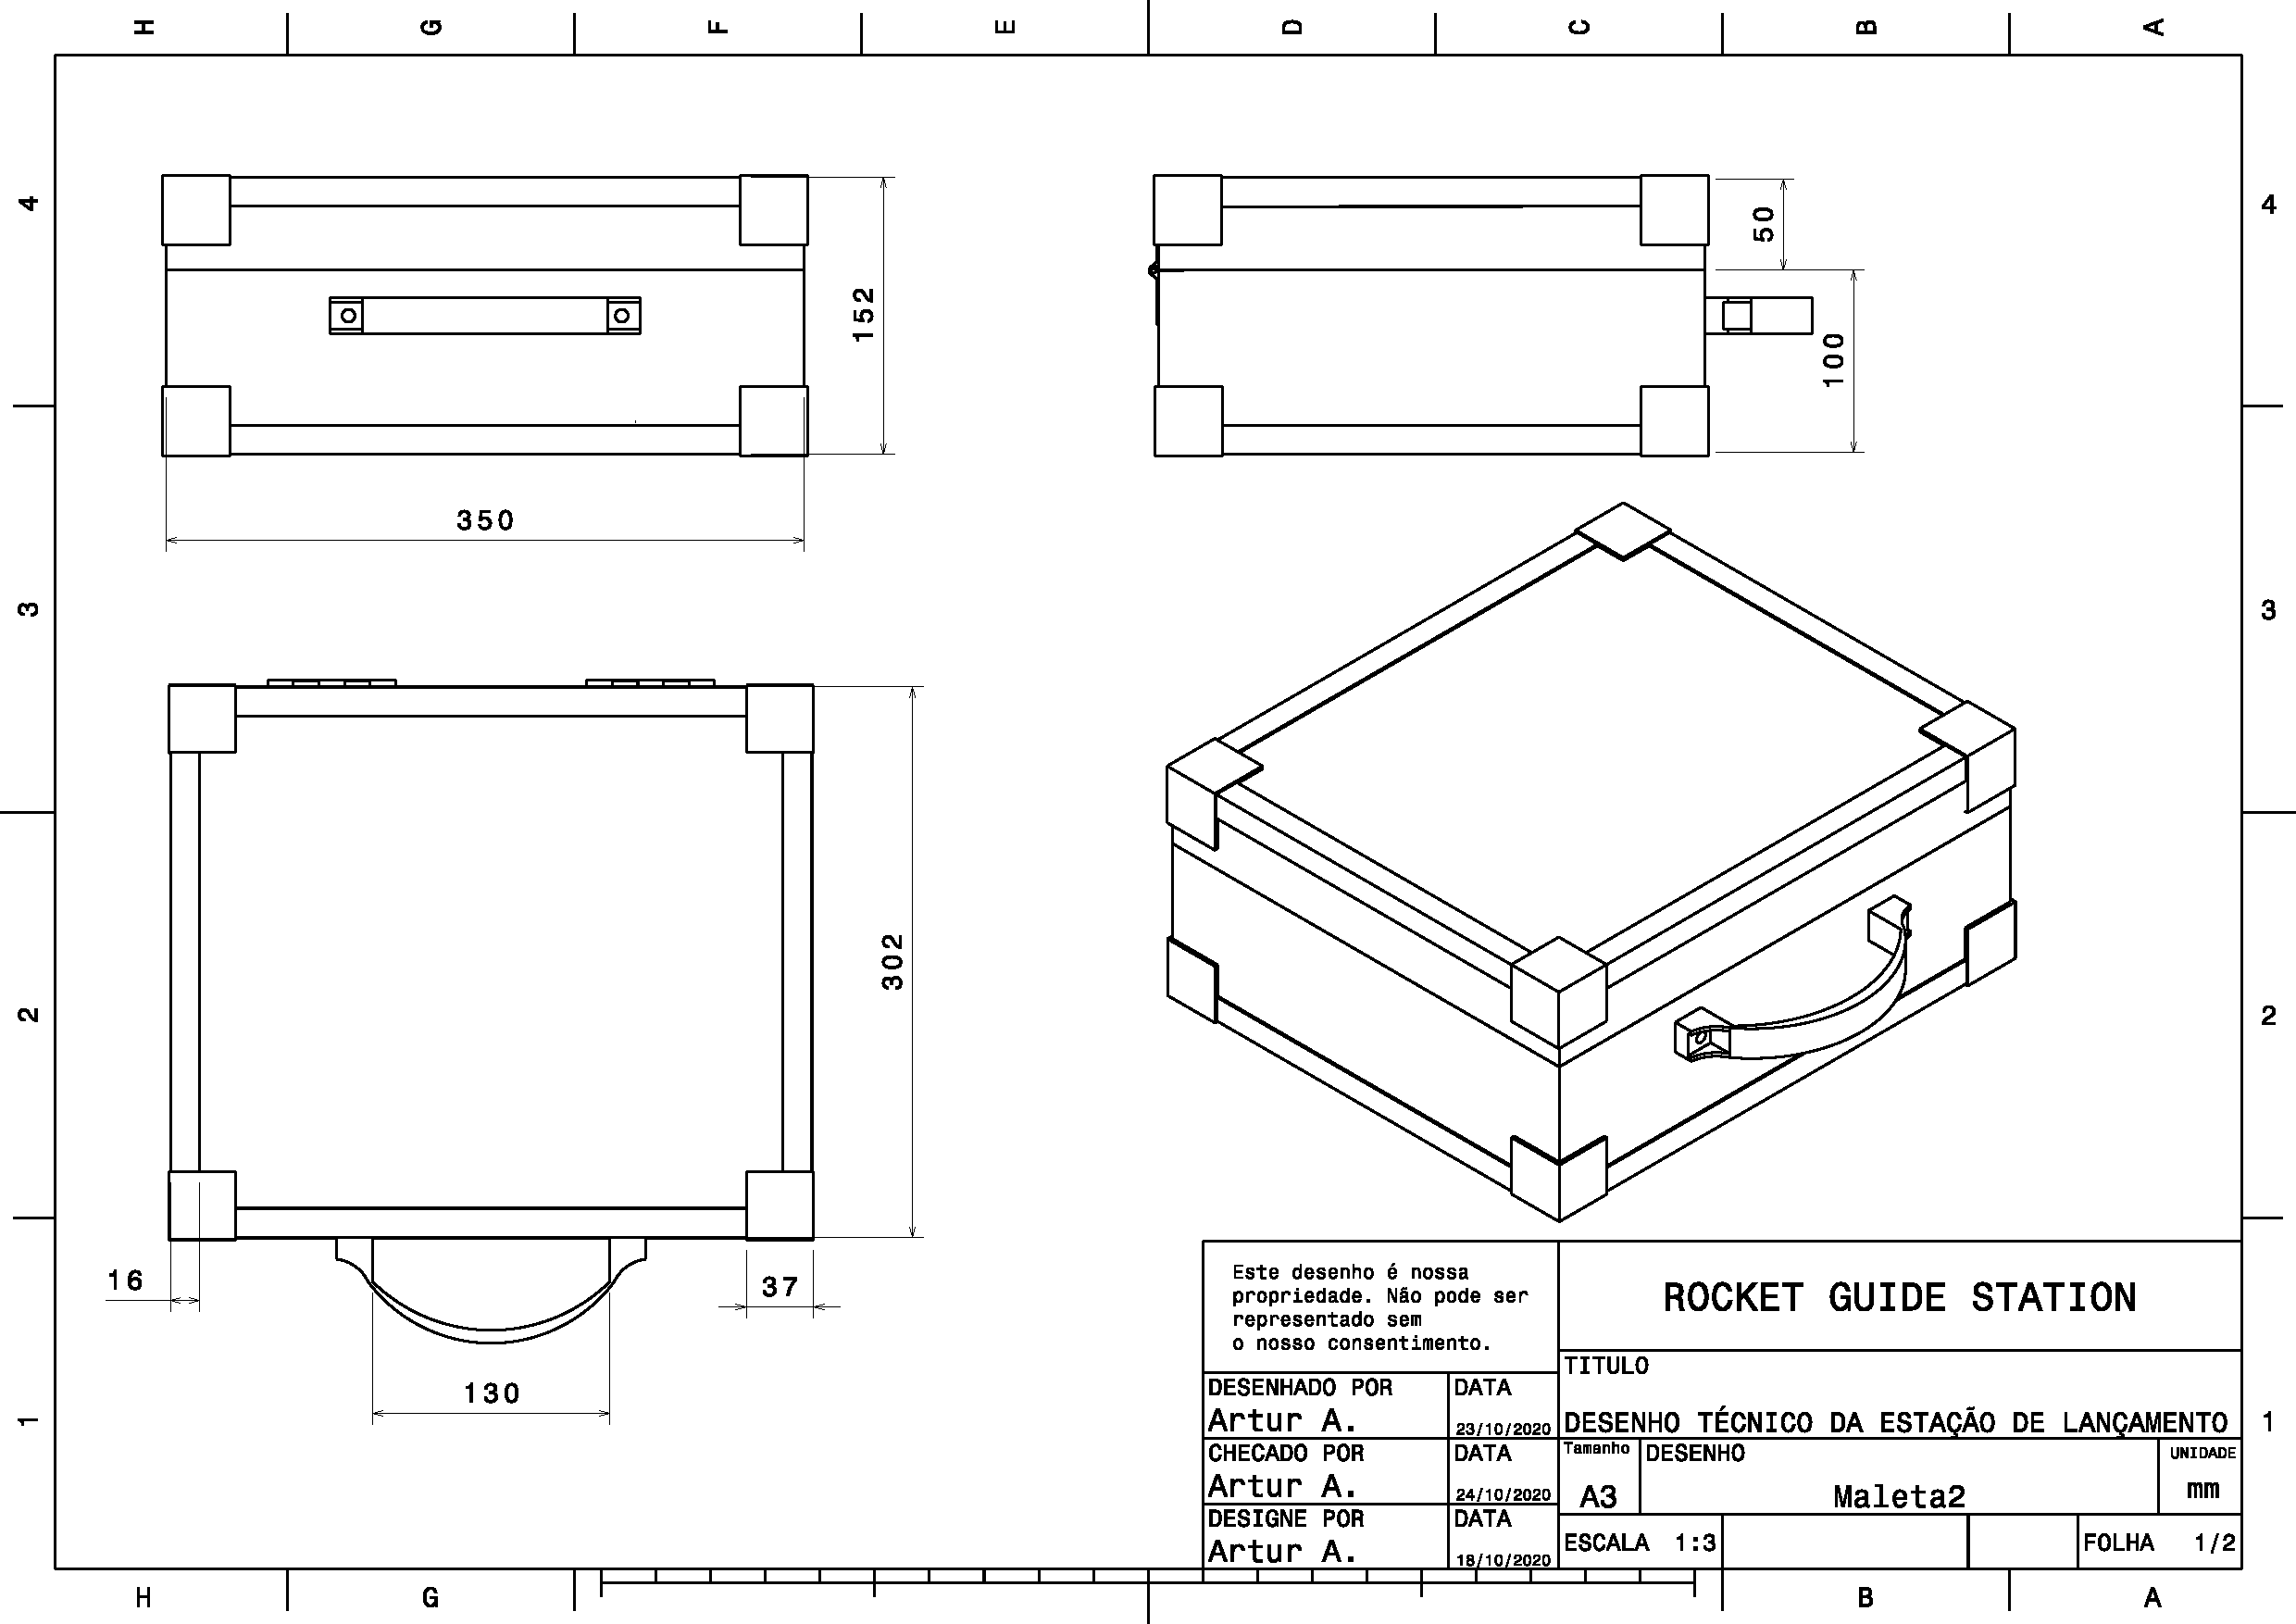
\includepdf[pages=-,angle=270]{figuras/PDFs/M2-1.pdf}
\label{GCS}


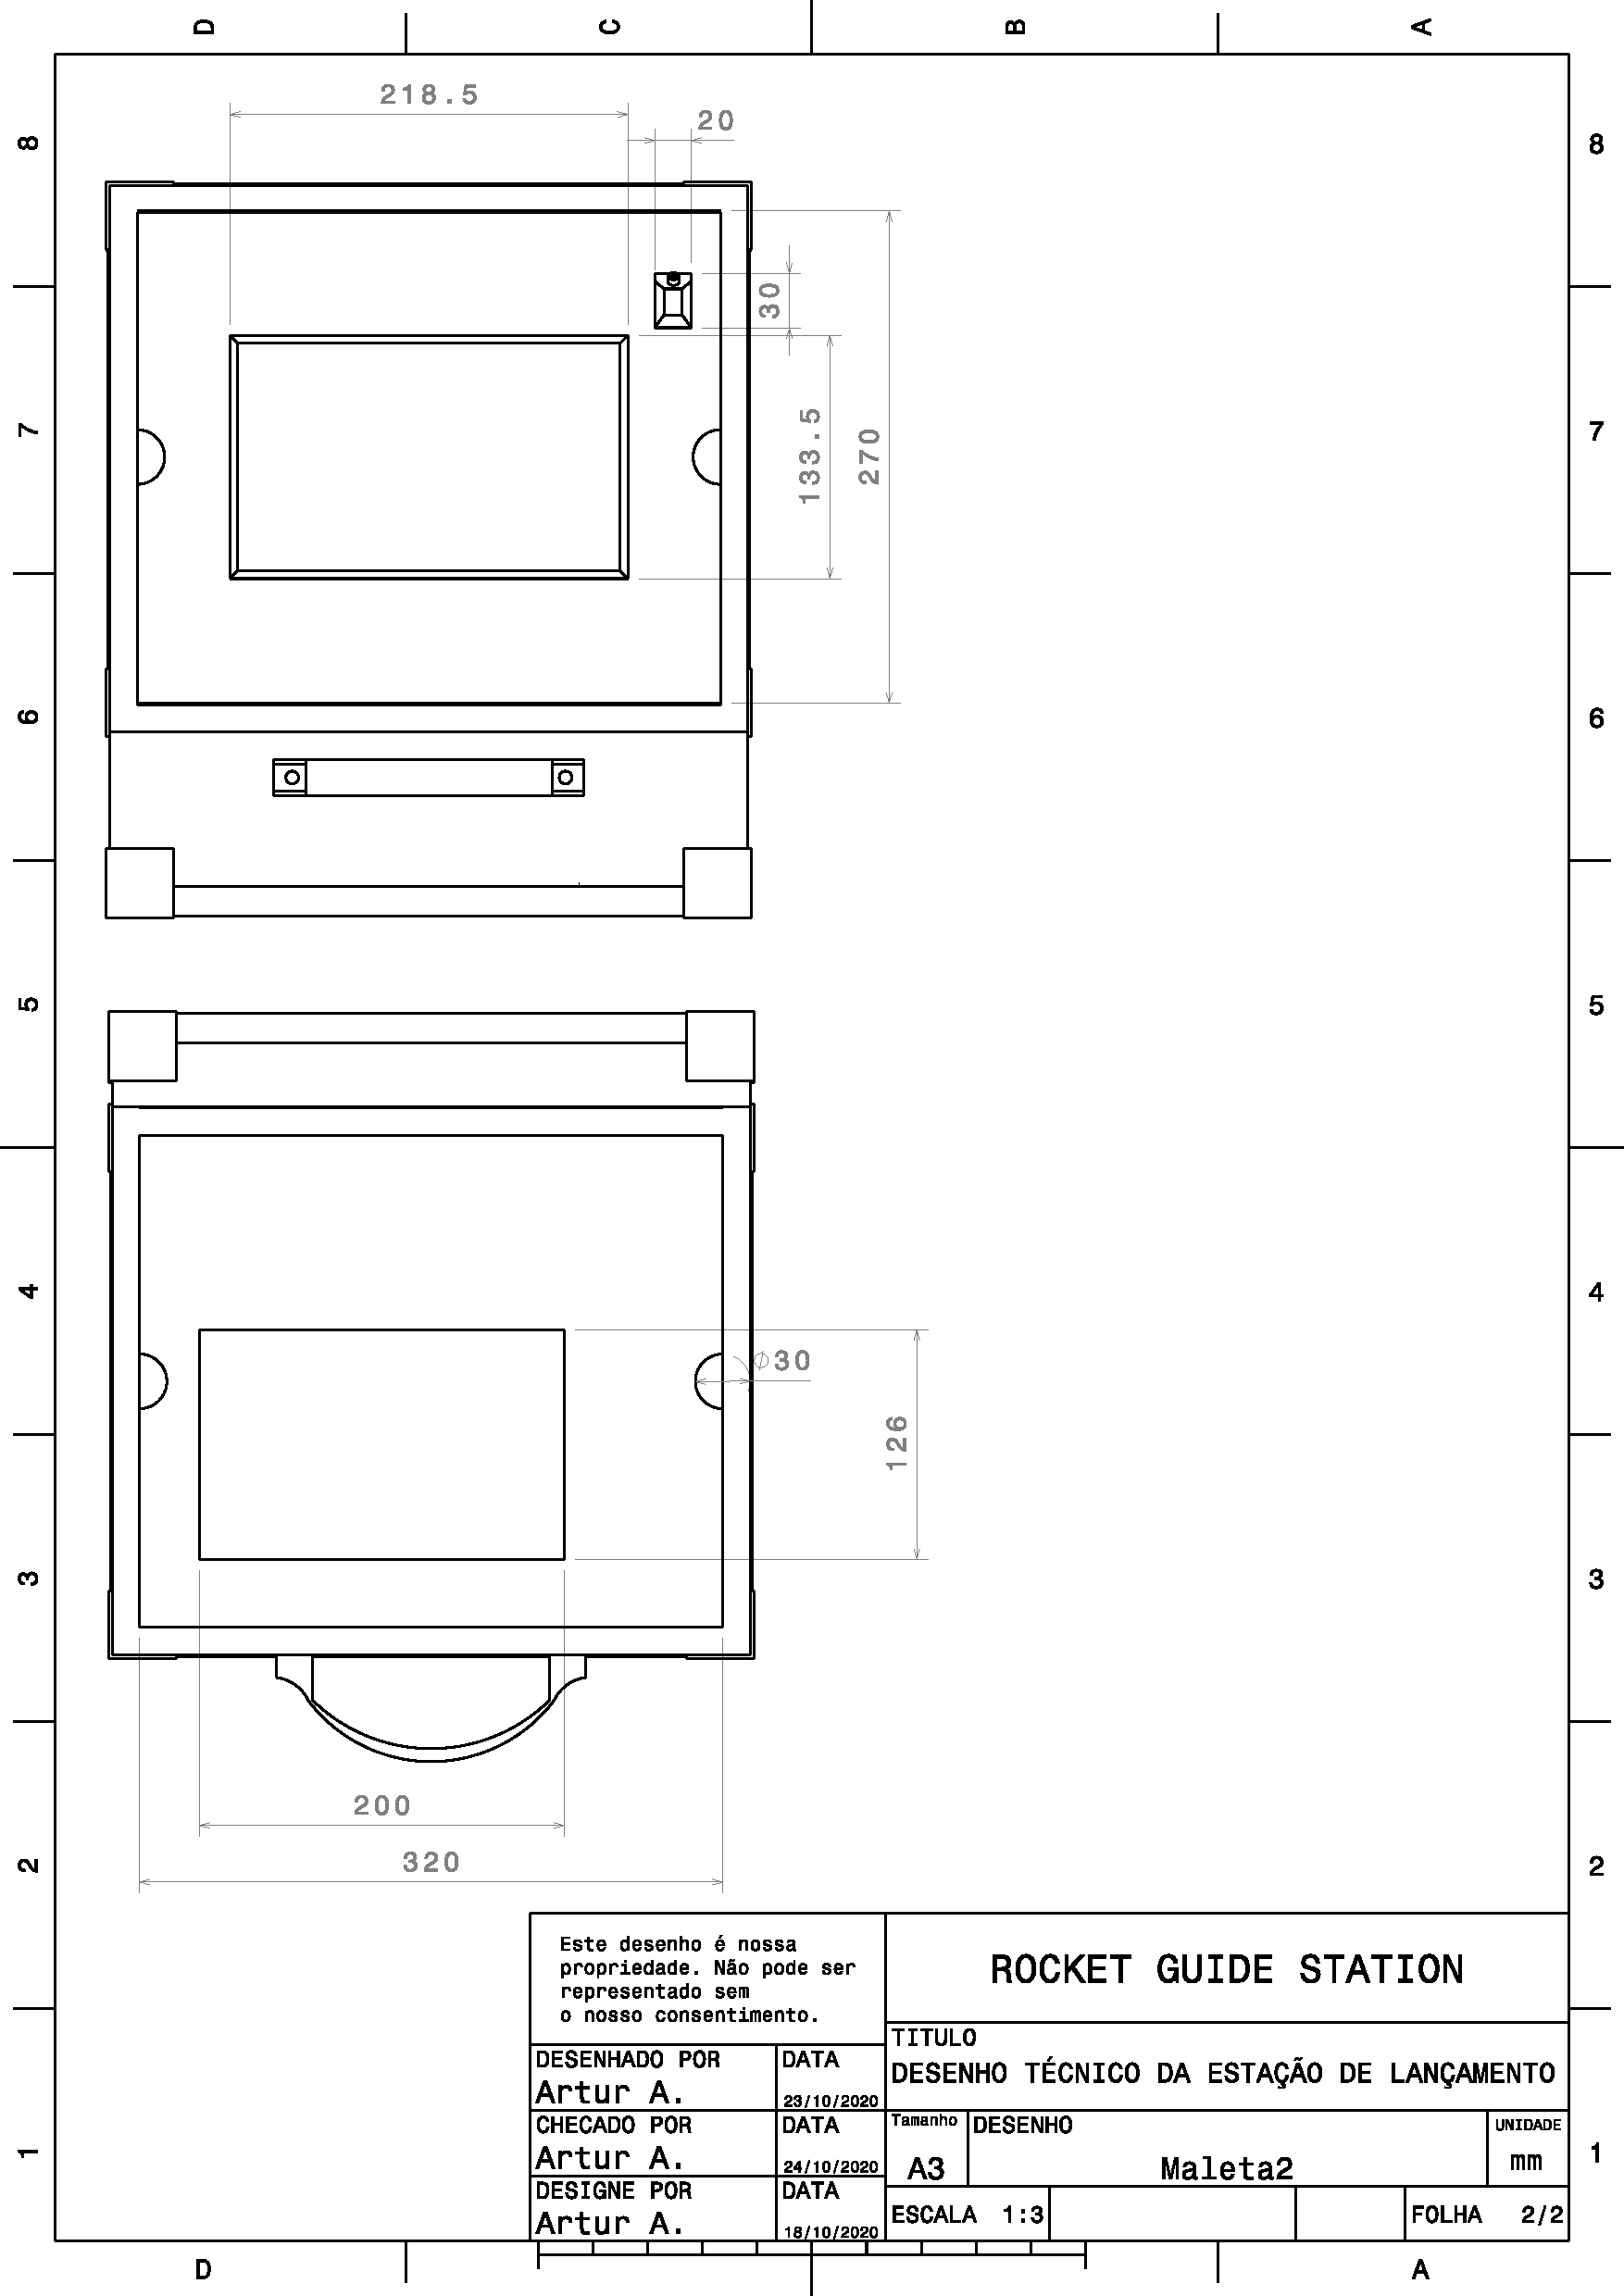
\includepdf[pages=-]{figuras/PDFs/M2-2.pdf}
\label{GCS1}

%\section{MaletaAbastecimento}

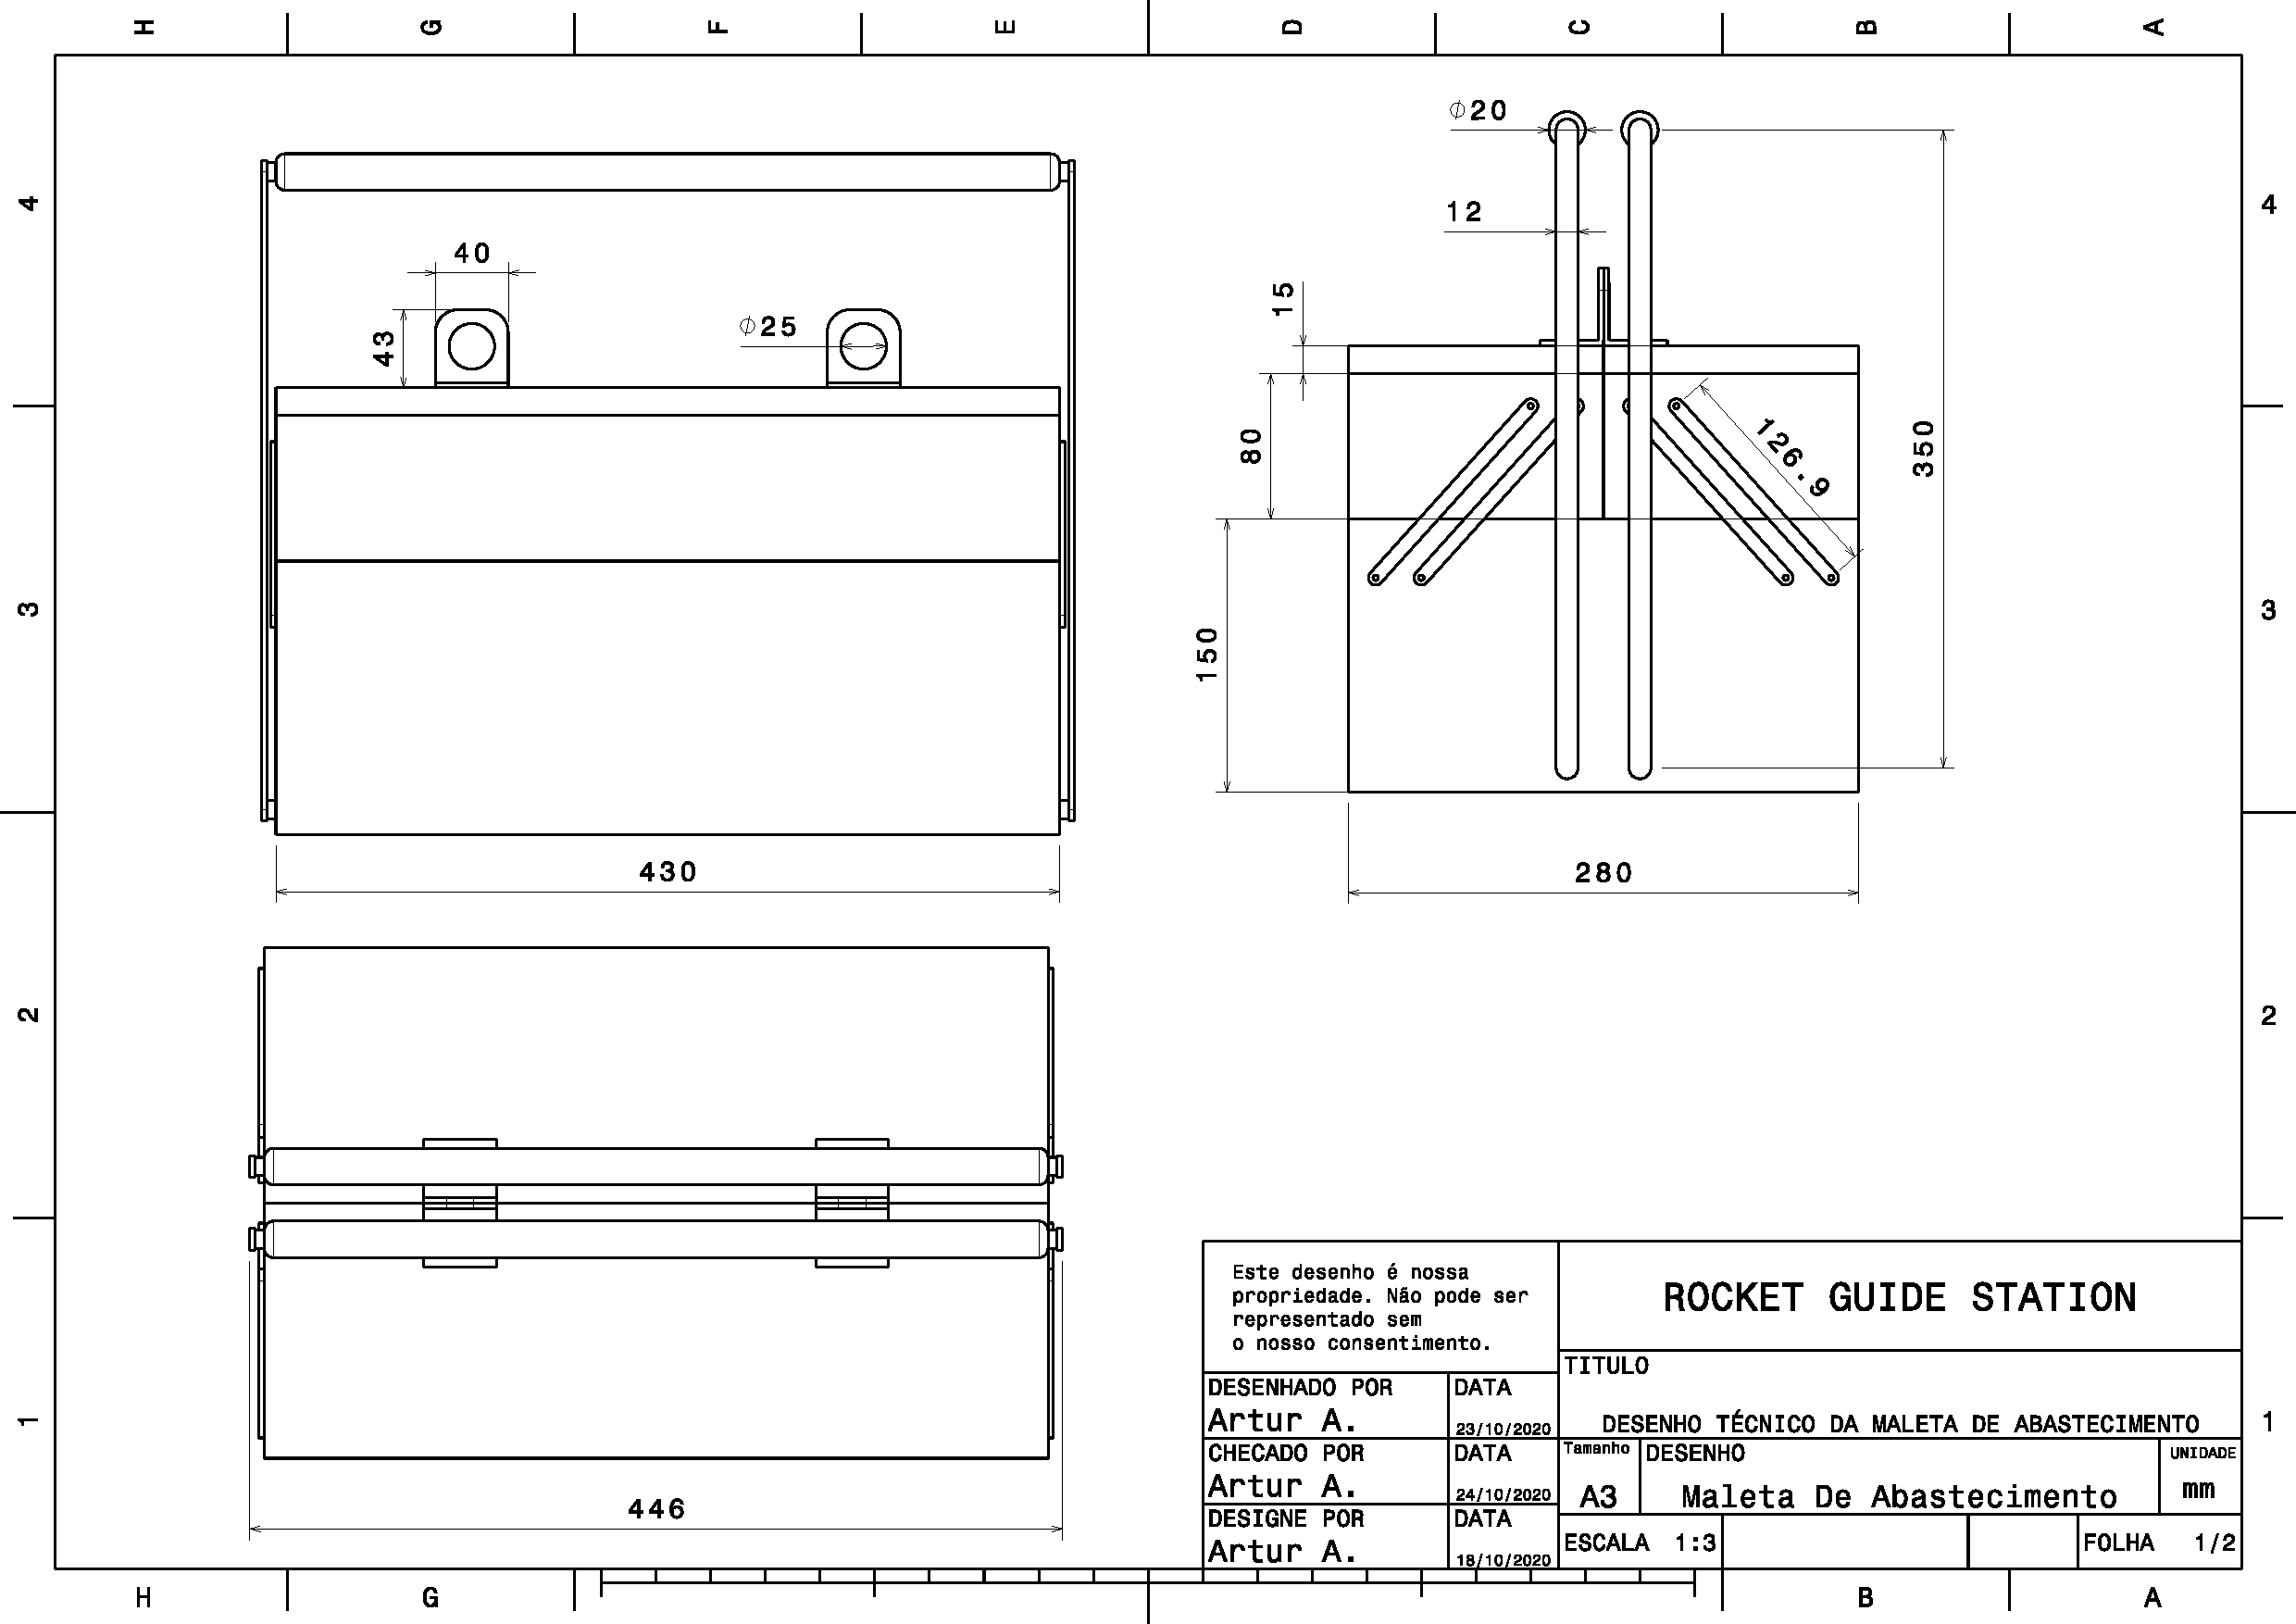
\includepdf[pages=-,angle=270]{figuras/PDFs/M3-1.pdf}
\label{MAbastecimento}


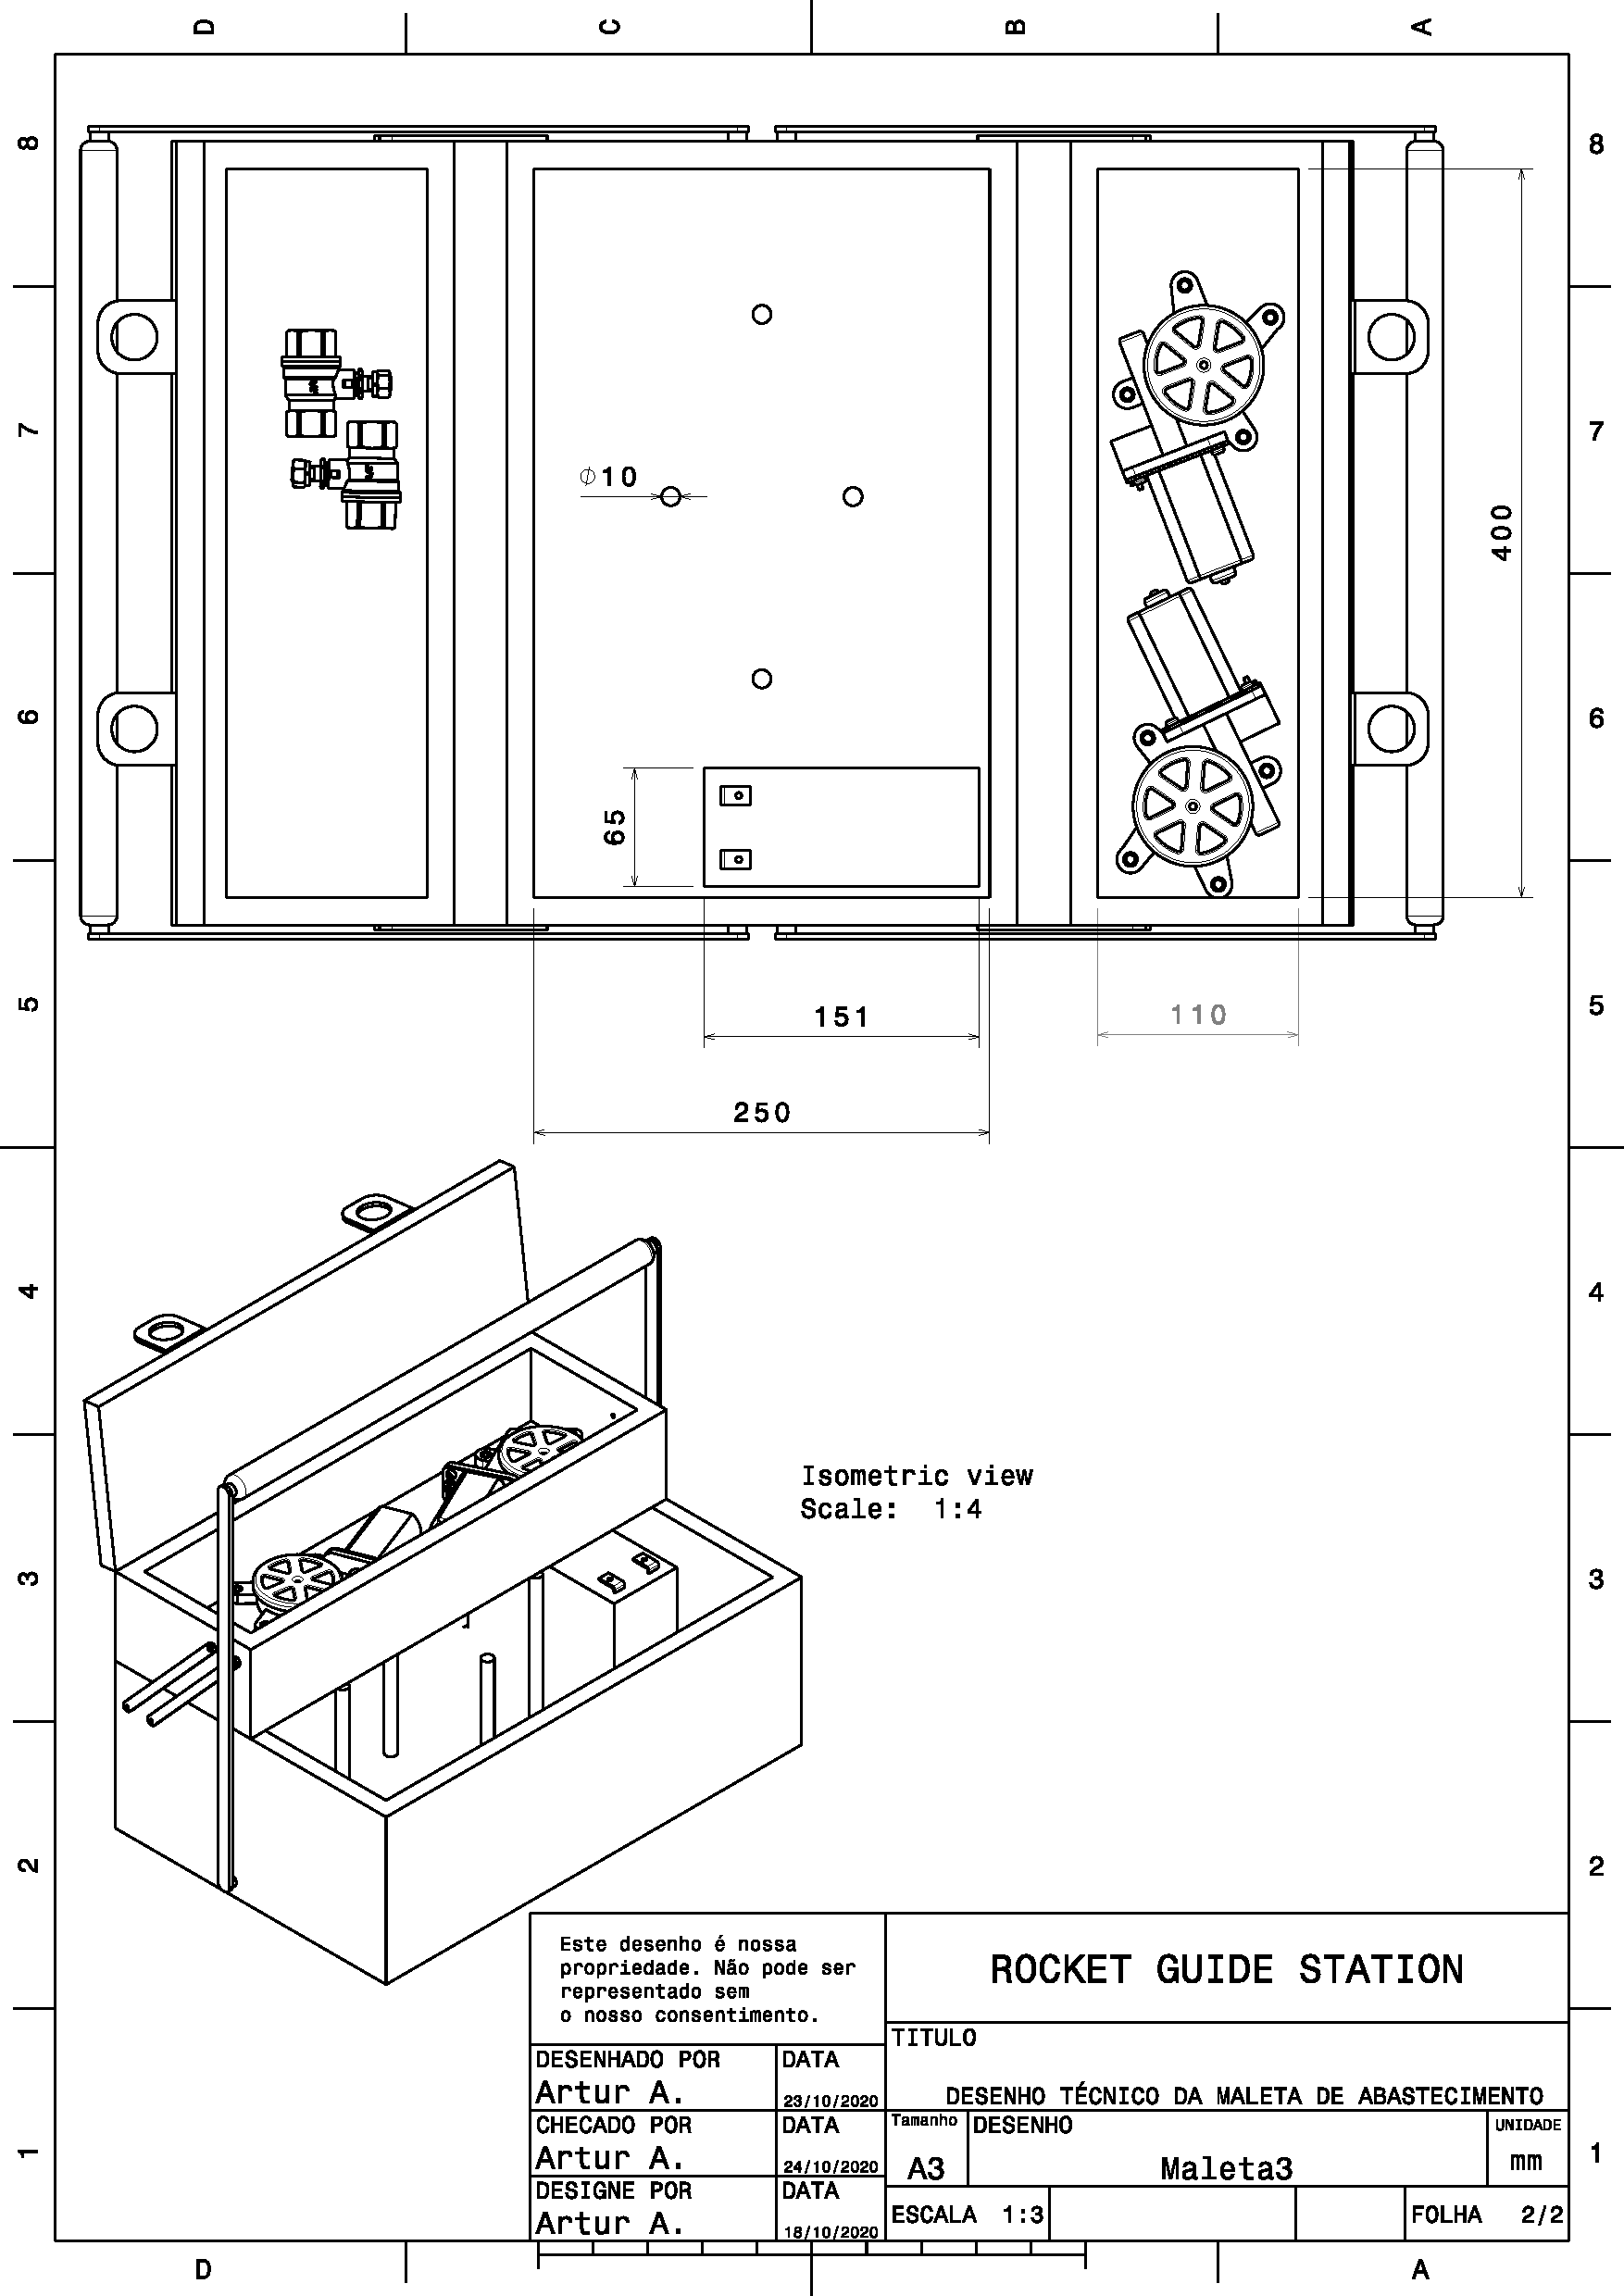
\includepdf[pages=-]{figuras/PDFs/M3-2.pdf}
\label{MAbastecimento1}

\chapter{Simulação de Impacto}
\label{simulacoes_impacto}

\begin{figure}[htb]
    \centering
    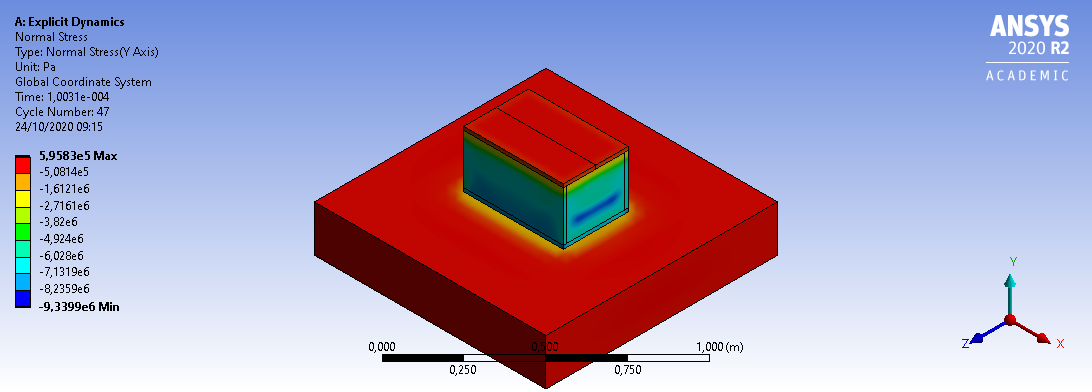
\includegraphics[width=1.0\textwidth, angle=0]{figuras/estrutura_simulacaoImpacto/ignicaoNormalYLadoMaior.png}
    \caption{Tensão normal no eixo Y da maleta do sistema de alimentação em queda direta}
    \label{fig:simulacaoImpacto_01}
\end{figure}

\begin{figure}[htb]
    \centering
    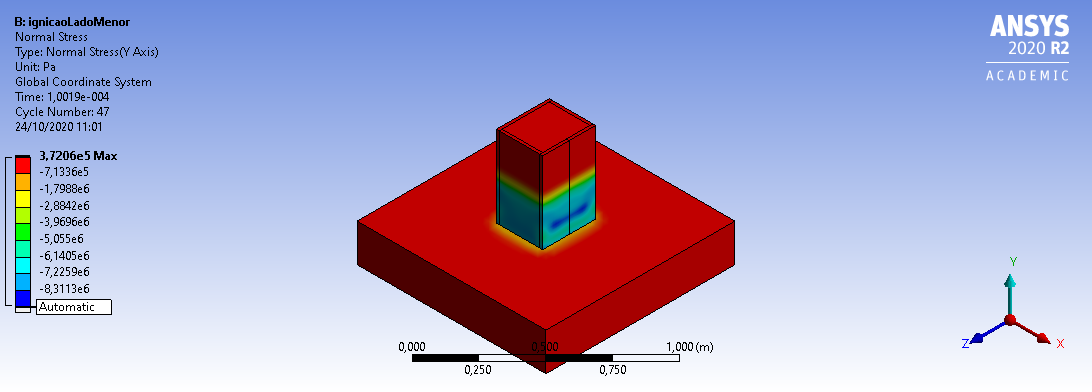
\includegraphics[width=1.0\textwidth, angle=0]{figuras/estrutura_simulacaoImpacto/ignicaoNormalYLadoMenor.png}
    \caption{Tensão normal no eixo Y da maleta do sistema de alimentação em queda lateral}
    \label{fig:simulacaoImpacto_02}
\end{figure}

\begin{figure}[htb]
    \centering
    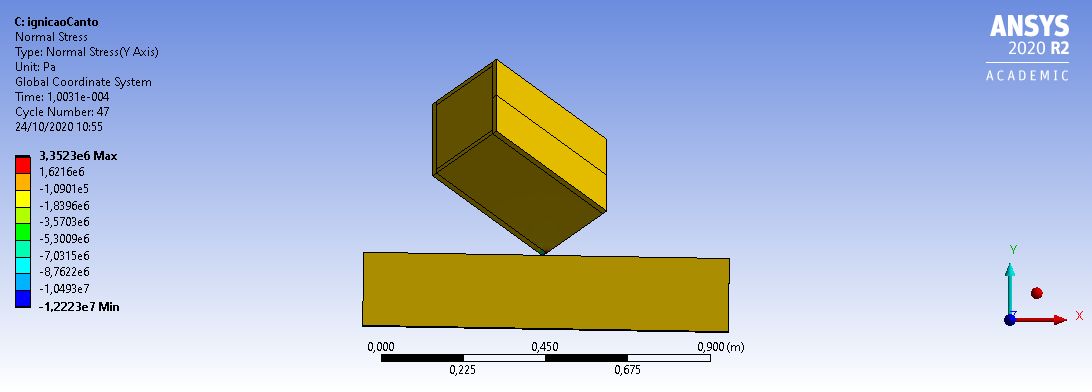
\includegraphics[width=1.0\textwidth, angle=0]{figuras/estrutura_simulacaoImpacto/ignicaoNormalYCanto.png}
    \caption{Tensão normal no eixo Y da maleta do sistema de alimentação em queda inclinada}
    \label{fig:simulacaoImpacto_03}
\end{figure}


\begin{figure}[htb]
    \centering
    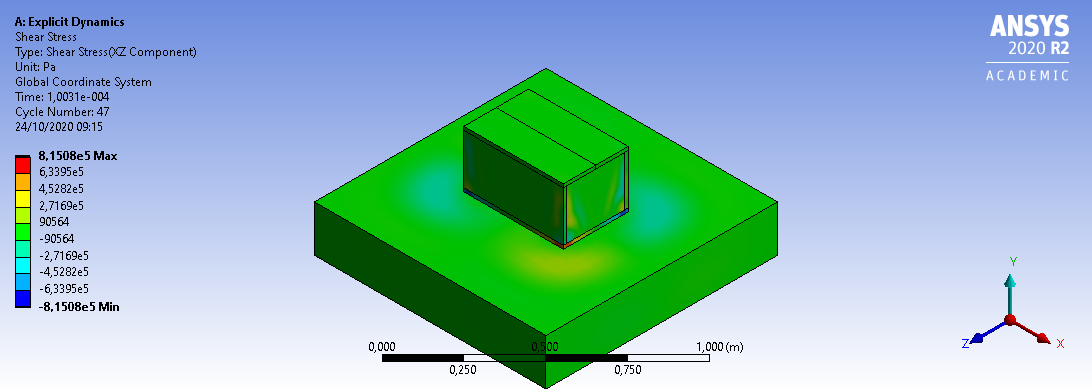
\includegraphics[width=1.0\textwidth, angle=0]{figuras/estrutura_simulacaoImpacto/ignicaoCisalhamentoXZLadoMaior.png}
    \caption{Tensão de Cisalhamento no plano XZ da maleta do sistema de alimentação em queda direta}
    \label{fig:simulacaoImpacto_04}
\end{figure}

\begin{figure}[htb]
    \centering
    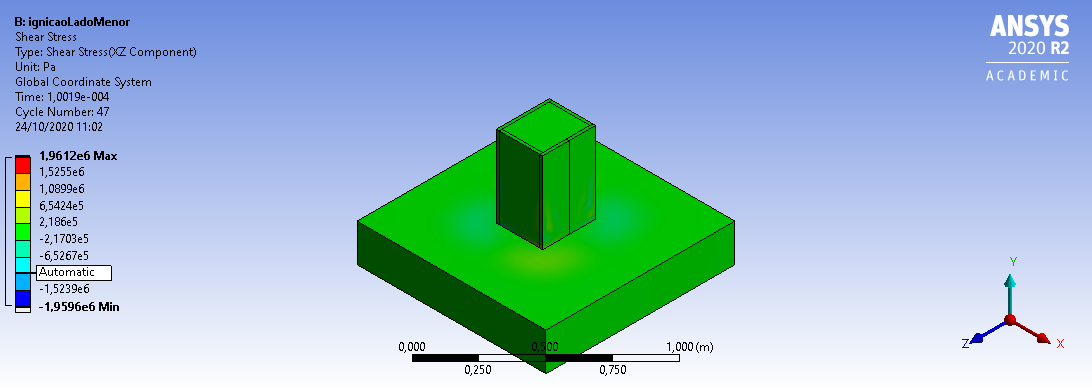
\includegraphics[width=1.0\textwidth, angle=0]{figuras/estrutura_simulacaoImpacto/ignicaoCisalhamentoXZLadoMenor.png}
    \caption{Tensão de Cisalhamento no plano XZ da maleta do sistema de alimentação em queda lateral}
    \label{fig:simulacaoImpacto_05}
\end{figure}

\begin{figure}[htb]
    \centering
    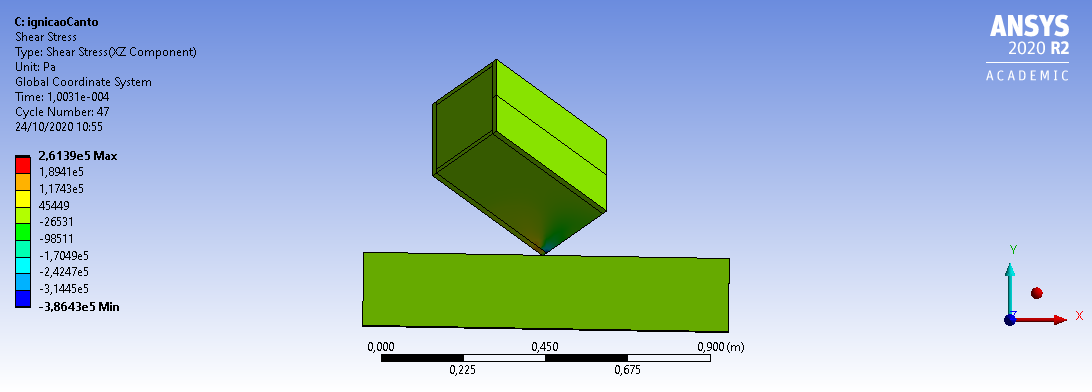
\includegraphics[width=1.0\textwidth, angle=0]{figuras/estrutura_simulacaoImpacto/ignicaoCisalhamentoXZCanto.png}
    \caption{Tensão de Cisalhamento no plano XZ da maleta do sistema de alimentação em queda inclinada}
    \label{fig:simulacaoImpacto_06}
\end{figure}

\begin{figure}[htb]
    \centering
    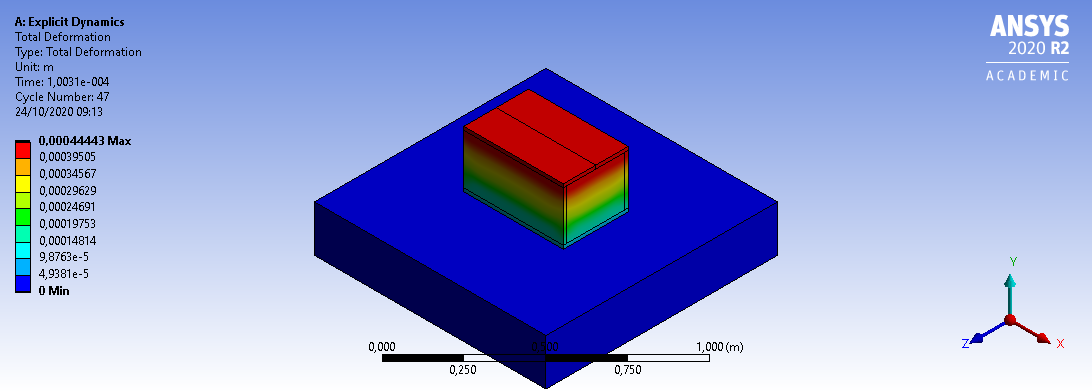
\includegraphics[width=1.0\textwidth, angle=0]{figuras/estrutura_simulacaoImpacto/ignicaoDeformacaoLadoMaior.png}
    \caption{Deformação da maleta do sistema de alimentação em queda direta}
    \label{fig:simulacaoImpacto_07}
\end{figure}

\begin{figure}[htb]
    \centering
    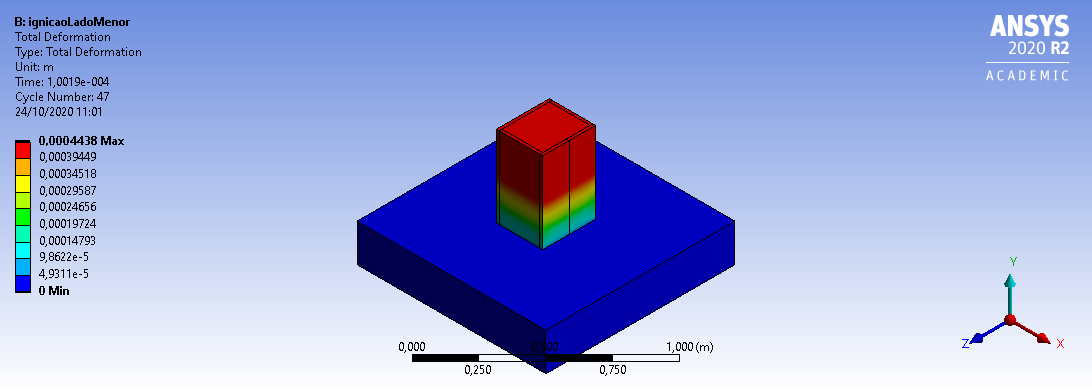
\includegraphics[width=1.0\textwidth, angle=0]{figuras/estrutura_simulacaoImpacto/ignicaoDeformacaoLadoMenor.png}
    \caption{Deformação da maleta do sistema de alimentação em queda lateral}
    \label{fig:simulacaoImpacto_08}
\end{figure}

\begin{figure}[htb]
    \centering
    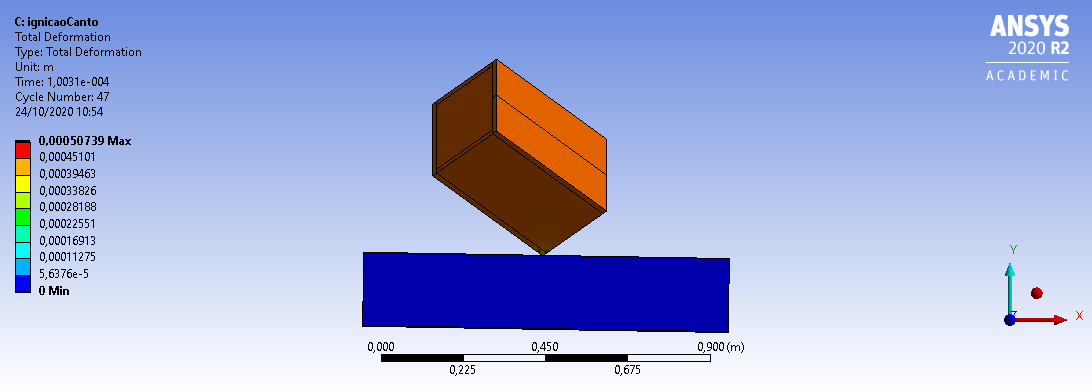
\includegraphics[width=1.0\textwidth, angle=0]{figuras/estrutura_simulacaoImpacto/ignicaoDeformacaoCanto.png}
    \caption{Deformação da maleta do sistema de alimentação em queda inclinada}
    \label{fig:simulacaoImpacto_09}
\end{figure}

\begin{figure}[htb]
    \centering
    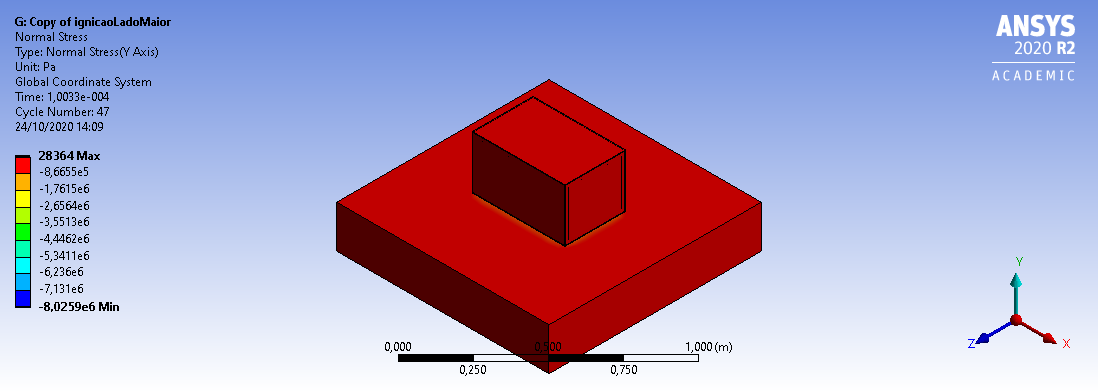
\includegraphics[width=1.0\textwidth, angle=0]{figuras/estrutura_simulacaoImpacto/ignicaoRevestidaNormalYMaior.png}
    \caption{Tensão normal no eixo Y da maleta do sistema de alimentação revestida em queda direta}
    \label{fig:simulacaoImpacto_10}
\end{figure}

\begin{figure}[htb]
    \centering
    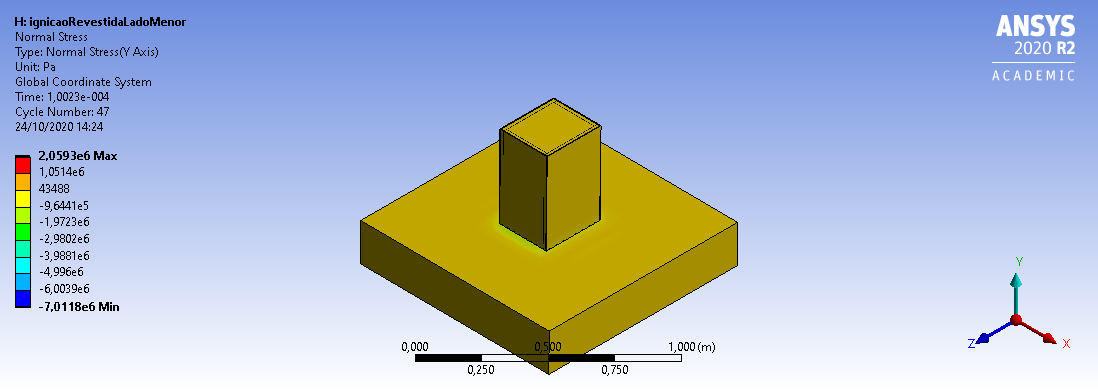
\includegraphics[width=1.0\textwidth, angle=0]{figuras/estrutura_simulacaoImpacto/ignicaoRevestidaNormalYMenor.png}
    \caption{Tensão normal no eixo Y da maleta do sistema de alimentação revestida em queda lateral}
    \label{fig:simulacaoImpacto_11}
\end{figure}

\begin{figure}[htb]
    \centering
    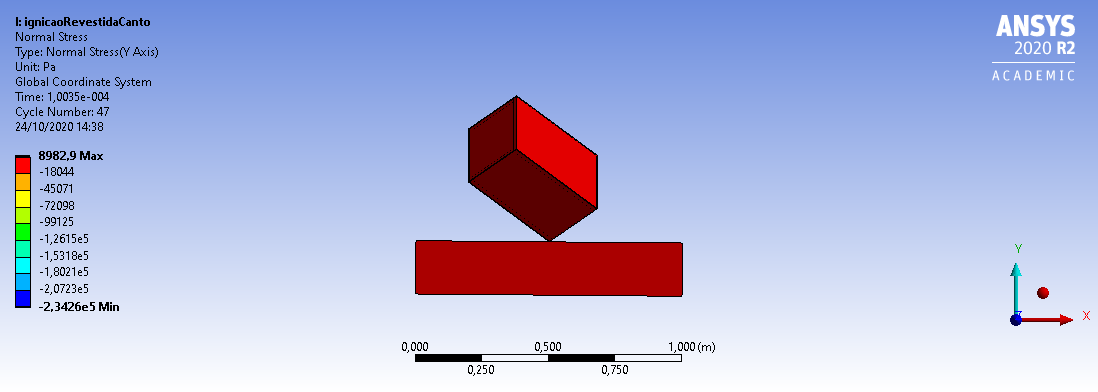
\includegraphics[width=1.0\textwidth, angle=0]{figuras/estrutura_simulacaoImpacto/ignicaoRevestidaNormalYCanto.png}
    \caption{Tensão normal no eixo Y da maleta do sistema de alimentação revestida em queda inclinada}
    \label{fig:simulacaoImpacto_12}
\end{figure}

\begin{figure}[htb]
    \centering
    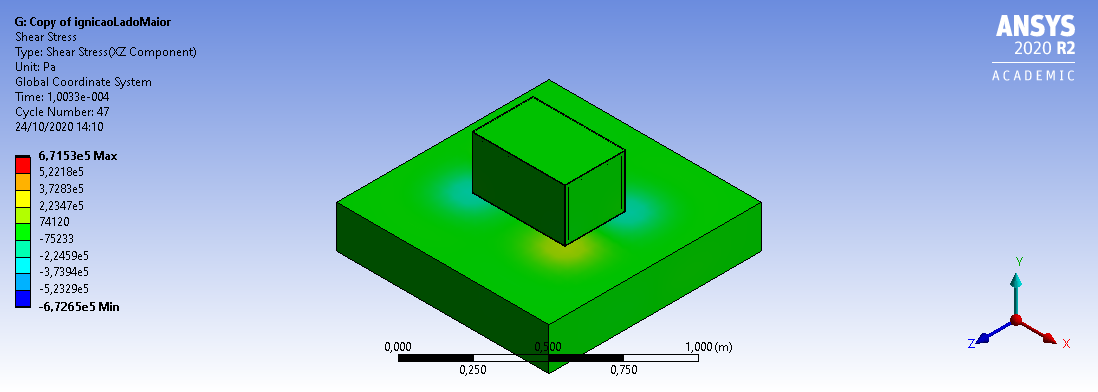
\includegraphics[width=1.0\textwidth, angle=0]{figuras/estrutura_simulacaoImpacto/ignicaoRevestidaCisalhamentoXZMaior.png}
    \caption{Tensão de cisalhamento no plano XZ da maleta do sistema de alimentação revestida em queda direta}
    \label{fig:simulacaoImpacto_13}
\end{figure}

\begin{figure}[htb]
    \centering
    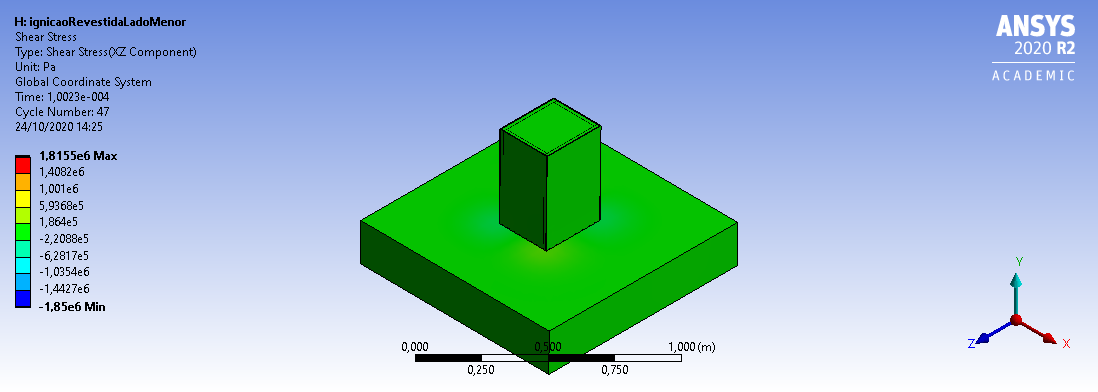
\includegraphics[width=1.0\textwidth, angle=0]{figuras/estrutura_simulacaoImpacto/ignicaoRevestidaCisalhamentoXZMenor.png}
    \caption{Tensão de cisalhamento no plano XZ da maleta do sistema de alimentação revestida em queda lateral}
    \label{fig:simulacaoImpacto_14}
\end{figure}

\begin{figure}[htb]
    \centering
    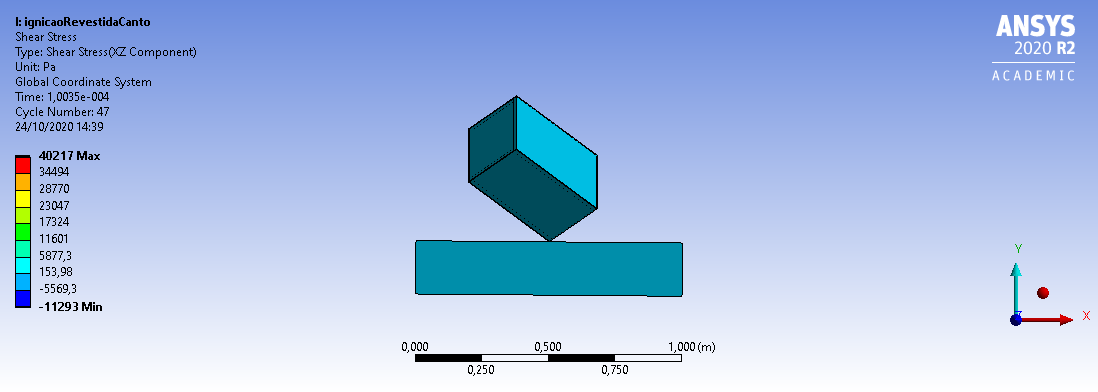
\includegraphics[width=1.0\textwidth, angle=0]{figuras/estrutura_simulacaoImpacto/ignicaoRevestidaCisalhamentoXZCanto.png}
    \caption{Tensão de cisalhamento no plano XZ da maleta do sistema de alimentação revestida em queda inclinada}
    \label{fig:simulacaoImpacto_15}
\end{figure}

\begin{figure}[htb]
    \centering
    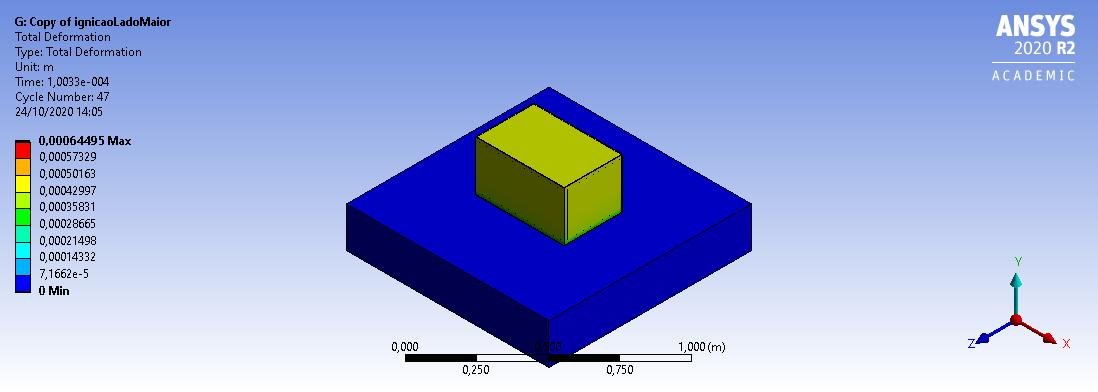
\includegraphics[width=1.0\textwidth, angle=0]{figuras/estrutura_simulacaoImpacto/ignicaoRevestidaDeformacaoMaior.png}
    \caption{Deformação da maleta do sistema de alimentação revestida em queda direta}
    \label{fig:simulacaoImpacto_16}
\end{figure}

\begin{figure}[htb]
    \centering
    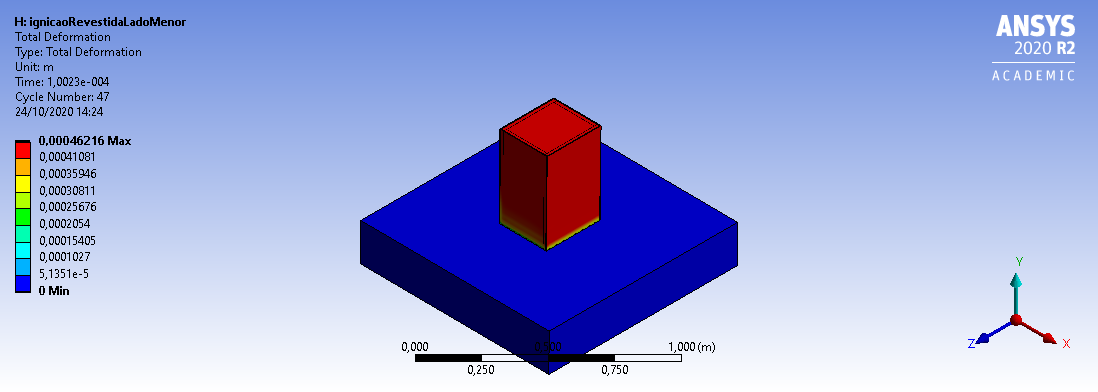
\includegraphics[width=1.0\textwidth, angle=0]{figuras/estrutura_simulacaoImpacto/ignicaoRevestidaDeformacaoMenor.png}
    \caption{Deformação da maleta do sistema de alimentação revestida em queda lateral}
    \label{fig:simulacaoImpacto_17}
\end{figure}

\begin{figure}[htb]
    \centering
    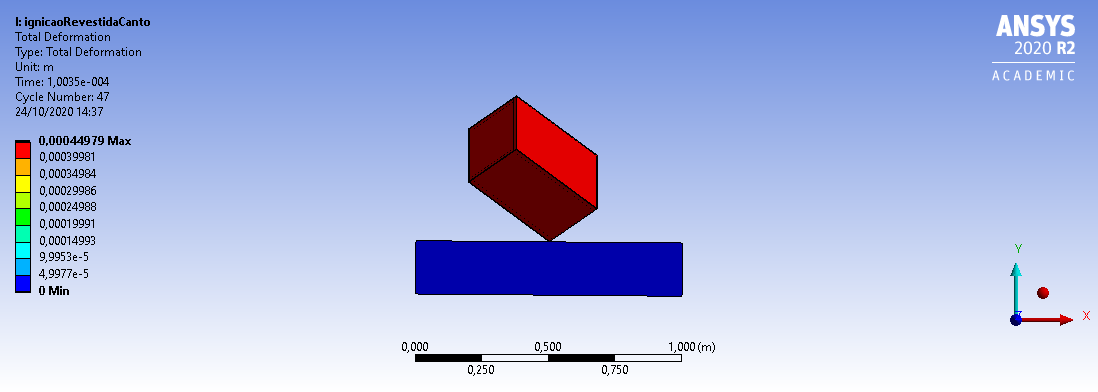
\includegraphics[width=1.0\textwidth, angle=0]{figuras/estrutura_simulacaoImpacto/ignicaoRevestidaDeformacaoCanto.png}
    \caption{Deformação da maleta do sistema de alimentação revestida em queda inclinada}
    \label{fig:simulacaoImpacto_18}
\end{figure}

\begin{figure}[htb]
    \centering
    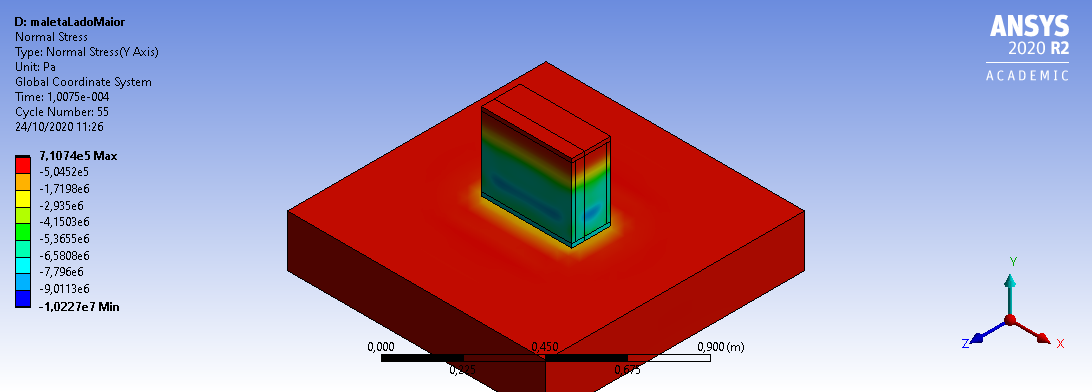
\includegraphics[width=1.0\textwidth, angle=0]{figuras/estrutura_simulacaoImpacto/maletaNormalYMaior.png}
    \caption{Tensão normal no eixo Y da maleta do sistema de controle em queda direta}
    \label{fig:simulacaoImpacto_19}
\end{figure}

\begin{figure}[htb]
    \centering
    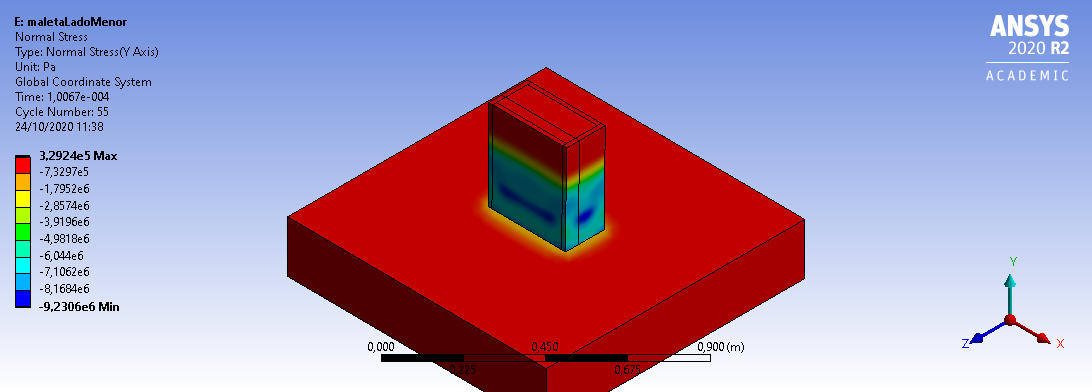
\includegraphics[width=1.0\textwidth, angle=0]{figuras/estrutura_simulacaoImpacto/maletaNormalYMenor.png}
    \caption{Tensão normal no eixo Y da maleta do sistema de controle em queda lateral}
    \label{fig:simulacaoImpacto_20}
\end{figure}

\begin{figure}[htb]
    \centering
    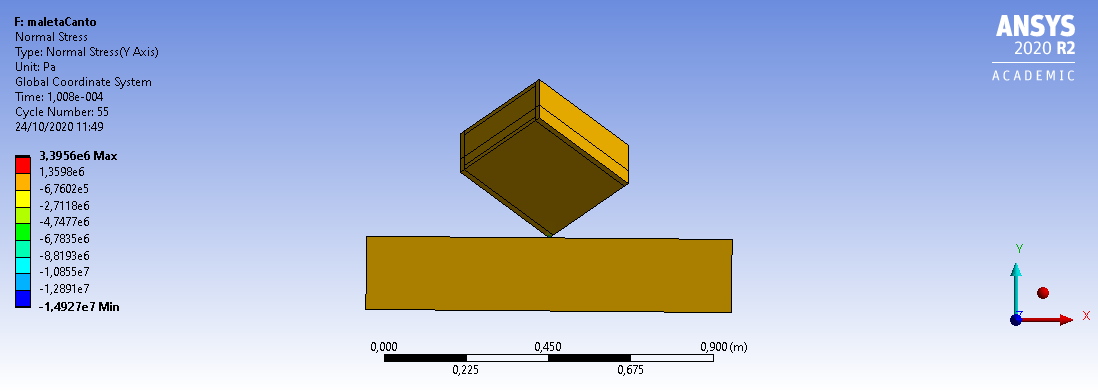
\includegraphics[width=1.0\textwidth, angle=0]{figuras/estrutura_simulacaoImpacto/maletaNormalYCanto.png}
    \caption{Tensão normal no eixo Y da maleta do sistema de controle em queda inclinada}
    \label{fig:simulacaoImpacto_21}
\end{figure}

\begin{figure}[htb]
    \centering
    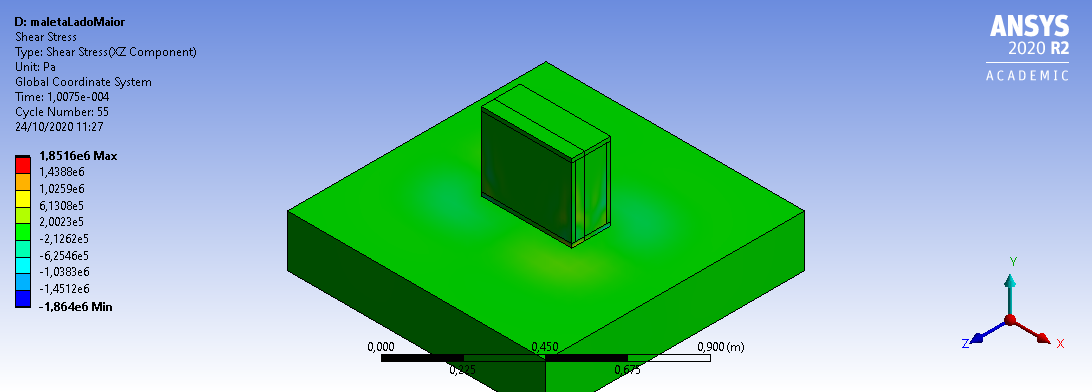
\includegraphics[width=1.0\textwidth, angle=0]{figuras/estrutura_simulacaoImpacto/maletaCisalhamentoXZMaior.png}
    \caption{Tensão de cisalhamento no plano XZ da maleta do sistema de controle em queda direta}
    \label{fig:simulacaoImpacto_22}
\end{figure}

\begin{figure}[htb]
    \centering
    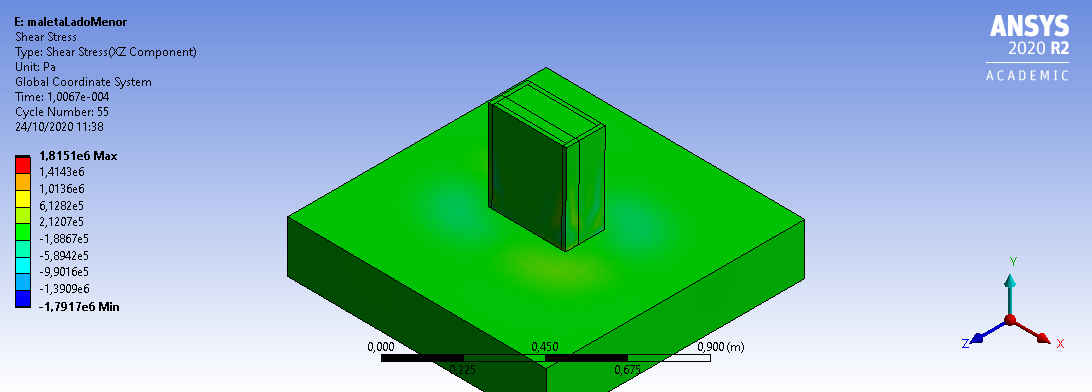
\includegraphics[width=1.0\textwidth, angle=0]{figuras/estrutura_simulacaoImpacto/maletaCisalhamentoXZMenor.png}
    \caption{Tensão de cisalhamento no plano XZ da maleta do sistema de controle em queda lateral}
    \label{fig:simulacaoImpacto_23}
\end{figure}

\begin{figure}[htb]
    \centering
    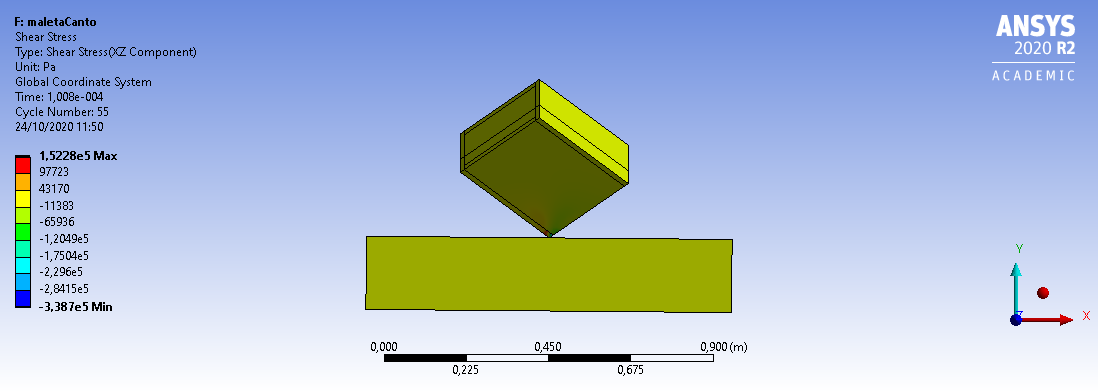
\includegraphics[width=1.0\textwidth, angle=0]{figuras/estrutura_simulacaoImpacto/maletaCisalhamentoXZCanto.png}
    \caption{Tensão de cisalhamento no plano XZ da maleta do sistema de controle em queda inclinada}
    \label{fig:simulacaoImpacto_24}
\end{figure}

\begin{figure}[htb]
    \centering
    \includegraphics[width=1.0\textwidth, angle=0]{figuras/estrutura_simulacaoImpacto/maletaDeformacaoMaior.png}
    \caption{Deformação da maleta do sistema de controle em queda direta}
    \label{fig:simulacaoImpacto_25}
\end{figure}

\begin{figure}[htb]
    \centering
    \includegraphics[width=1.0\textwidth, angle=0]{figuras/estrutura_simulacaoImpacto/maletaDeformacaoMenor.png}
    \caption{Deformação da maleta do sistema de controle em queda lateral}
    \label{fig:simulacaoImpacto_26}
\end{figure}

\begin{figure}[htb]
    \centering
    \includegraphics[width=1.0\textwidth, angle=0]{figuras/estrutura_simulacaoImpacto/maletaDeformacaoCanto.png}
    \caption{Deformação da maleta do sistema de controle em queda inclinada}
    \label{fig:simulacaoImpacto_27}
\end{figure}

\begin{figure}[htb]
    \centering
    \includegraphics[width=1.0\textwidth, angle=0]{figuras/estrutura_simulacaoImpacto/maletaRevestidaNormalYMaior.png}
    \caption{Tensão normal Y da maleta revestida do sistema de controle em queda direta}
    \label{fig:simulacaoImpacto_28}
\end{figure}

\begin{figure}[htb]
    \centering
    \includegraphics[width=1.0\textwidth, angle=0]{figuras/estrutura_simulacaoImpacto/maletaRevestidaNormalYMenor.png}
    \caption{Tensão normal Y da maleta revestida do sistema de controle em queda lateral}
    \label{fig:simulacaoImpacto_29}
\end{figure}

\begin{figure}[htb]
    \centering
    \includegraphics[width=1.0\textwidth, angle=0]{figuras/estrutura_simulacaoImpacto/maletaRevestidaNormalYCanto.png}
    \caption{Tensão normal Y da maleta revestida do sistema de controle em queda inclinada}
    \label{fig:simulacaoImpacto_30}
\end{figure}

\begin{figure}[htb]
    \centering
    \includegraphics[width=1.0\textwidth, angle=0]{figuras/estrutura_simulacaoImpacto/maletaRevestidaCisalhamentoXZMaior.png}
    \caption{Tensão de cisalhamento no plano XZ da maleta revestida do sistema de controle em queda direta}
    \label{fig:simulacaoImpacto_31}
\end{figure}

\begin{figure}[htb]
    \centering
    \includegraphics[width=1.0\textwidth, angle=0]{figuras/estrutura_simulacaoImpacto/maletaRevestidaCisalhamentoXZMenor.png}
    \caption{Tensão de cisalhamento no plano XZ da maleta revestida do sistema de controle em queda lateral}
    \label{fig:simulacaoImpacto_32}
\end{figure}

\begin{figure}[htb]
    \centering
    \includegraphics[width=1.0\textwidth, angle=0]{figuras/estrutura_simulacaoImpacto/maletaRevestidaCisalhamentoXZCanto.png}
    \caption{Tensão de cisalhamento no plano XZ da maleta revestida do sistema de controle em queda inclinada}
    \label{fig:simulacaoImpacto_33}
\end{figure}

\begin{figure}[htb]
    \centering
    \includegraphics[width=1.0\textwidth, angle=0]{figuras/estrutura_simulacaoImpacto/maletaRevestidaDeformationMaior.png}
    \caption{Deformação da maleta revestida do sistema de controle em queda direta}
    \label{fig:simulacaoImpacto_34}
\end{figure}

\begin{figure}[htb]
    \centering
    \includegraphics[width=1.0\textwidth, angle=0]{figuras/estrutura_simulacaoImpacto/maletaRevestidaDeformacaoMenor.png}
    \caption{Deformação da maleta revestida do sistema de controle em queda lateral}
    \label{fig:simulacaoImpacto_35}
\end{figure}

\begin{figure}[htb]
    \centering
    \includegraphics[width=1.0\textwidth, angle=0]{figuras/estrutura_simulacaoImpacto/maletaRevestidaDeformacaoCanto.png}
    \caption{Deformação da maleta revestida do sistema de controle em queda inclinada}
    \label{fig:simulacaoImpacto_36}
\end{figure}

\chapter[Registro de alterações]{Registro de alterações}
\label{alteracoes}


\begin{table}[H]
\centering
\begin{tabular}{|l|l|}
\hline
\textbf{Tópico de Referência} & \textbf{Descrição da Alterção} \\ \hline
Seção \ref{problema_solucao_antiga} & \begin{tabular}[c]{@{}l@{}}Estudo sobre as dificuldades de aplicar Aprendizado de Máquina \\ no projeto.\end{tabular} \\ \hline
Seção \ref{Peso_do_Foguete} &  \begin{tabular}[c]{@{}l@{}}Adição de mais uma célula de carga para medição do peso do \\   foguete.\end{tabular}\\ \hline


 &  \\ \hline
\end{tabular}
\caption{Lista de alterações significativas do projeto.}
\label{alteracoes}
\end{table}

\chapter[Autoavaliação]{Autoavaliação}
%\addcontentsline{toc}{chapter}{Contextualização}
\label{autoavaliacao}

\begin{itemize}

%    \item \textbf{Nome:Nome}
%    \begin{itemize}
%        \item 
%    \end{itemize}
    
    \item \textbf{Nome: Augusto Moreno Vilarins}
    \begin{itemize}
    \item Refinamento da definição do produto
    \item Levantamento de requisitos
    \item Storytelling
    \item Protótipo de baixa fidelidade
    \item Wireframe
    \item Reuniões de alinhamento com o cliente
    \item Protótipo de média fidelidade
    \item Auxilio na elaboração do documento do Ponto de Controle 2
    \item Correção das mudanças sugeridas para o documento do ponto de controle 2
    \item Revisão e edição do documento de ponto de controle 3
    \item Manual de usuário
    \item Manual de montagem
    \item Documentação das reuniões com clientes
    \item Preparação do ambiente de desenvolvimento do Front end
    \item Auxílio no desenvolvimento do front end
    \end{itemize}
    
    
    \item \textbf{Nome: Artur Cardoso de Almeida}
    \begin{itemize}
      \item Dimensionamento do case de eletrônica. 
      \item Dimensionamento do carregador de energia.
      \item Redimensionamento da estrutura da Maleta 02 - Abastecimento.
      \item Criação dos CADS das maletas.
      \item Criação do CAD da case de de eletrônica.
      \item Criação do CAD do carregador de energia.
      \item Criação dos desenhos técnicos das estruturas.
      \item Tabela de materiais com vista explodida.
      \item Alinhamento sobre a disposição dos componentes da central de controle com o grupo de eletrônica. 
      \item Integração com o subsistema de eletrônica.
      \item Integração com o subsistema de energia.
      \item Renderização da maleta GCS e da maleta de abastecimento.
      \item Renderização do case de eletrônica
      \item Renderização do carregador de energia.
      \item Renderização do sistema de abastecimento.
      \item Orçamento dos componentes para fabricação da maleta.
      \item Auxilio na definição da solução de acoplamento dos atuadores nas válvulas.
      \item Auxílio na edição e revisão do Ponto de Controle 3.
      \item Auxilio na confecção do manual de montagem.
      \item Auxilio na confecção do manual de usuário.
    \end{itemize}


    \item \textbf{Nome: Diogo Filipe Sens}
    \begin{itemize}
     \item Revisão da simulação de impacto.
     \item Elaboração do plano de montagem das estruturas das duas maletas.
     \item Definição dos elementos de fixação dos componentes estruturais das duas maletas.
     \item elaboração de desenhos que ilustrem a sequência de montagem das duas maletas.
     \item Confecção do manual de montagem sobre a parte estrutural da maleta.
     \item Auxílio na elaboração do \textit{case} de suporte do subsistema válvula + motor + adaptador.
    \end{itemize}

    
    \item \textbf{Nome: Douglas Alves Brandão}
    \begin{itemize}
         \item Definição dos requisitos da estrutura utilizada no protótipo.
         \item Definição dos possíveis materiais a serem utilizados na construção da Ground Station.
         \item Auxílio na elaboração dos CADs da maleta. 
         \item Detalhamento das características dos materiais a serem utilizados na construção da Ground Station.
         \item Auxílio na modelagem do sistema de abastecimento. 
         \item Auxílio na simulação do sistema de abastecimento no software Simulink/Matlab.
         \item Definição dos parâmetros do sistema de abastecimento.
        \item Definição da solução para a abertura de válvulas.
         \item Auxílio na elaboração dos documentos dos Pontos de Controles.
         \item Confecção das instruções para o manual de montagem.
        \item Confecção do manual de montagem.
        \item Confecção dos CADs do sistema de abastecimento.
    \end{itemize}


    \item \textbf{Nome: Gustavo Cavalcante Linhares}
    \begin{itemize}
         \item Gerenciamento e acompanhamento das atividades do grupo de eletrônica 
         \item Detalhamento da solução de integração entre hardware e eletrônica
         \item Alinhamento com os gerentes sobre as soluções tomadas e sobre o desenvolvimento do projeto
         \item Alinhamento entre eletrônica, sub áreas do projeto e o Stakeholder sobre as soluções que possuem impacto no trabalho em mais de um grupo dentro do projeto.
         \item Revisão final dos diagramas esquemático e do projeto de PCI's.
         \item Construção do Manual de montagem no subtópico da montagem dos componentes eletrônicos 
         \item Auxilio na construção do Manual de usuário
         \item Revisão da documentação do PC3 do manual de usuário e manual de montagem
    \end{itemize}
    
    
    \item \textbf{Nome: Francisco Matheus Fernandes Gomes}
    \begin{itemize}
     \item Revisão final dos diagramas esquemático e do projeto de PCI's.
    \item Criação do diagrama de blocos do abastecimento do projeto e no auxilio do diagrama geral.
    \item Auxílio na edição e revisão do Ponto de Controle 3.
    \item Confecção do manual de montagem.
    \item Confecção do manual do usuário.
   \item Levantamento e definição de requisito para o funcionamento da telemetria por Lora na ESP32.
   \item Auxílio na definição da solução de acionamento e controle eletrônico das válvulas internas e externas ao foguete.
    \item Auxílio na integração da eletrônica com os grupos de energia e estrutura.
    \item Atualização dos custos dos componentes que envolve o hardware do projeto.
    \end{itemize}
    
    \item \textbf{Nome: Gabriela Alves da Gama}
    \begin{itemize}
     \item Desenvolvimento do Manter Hardware e Comando;
    \item Configuração do banco de dados;
    \item Desenvolvimento do Manter Foguete;
    \item Desenvolvimento do calculo de velocidade;
    \item Desenvolvimento do manter altitude, gps, missao, peso, pressão, e velocidade; 
    \item Descrever construção do backend;
    \item Desenvolvimento do serviço de simulação
    \item Revisão dos artefatos de software
    \end{itemize}

    
    \item \textbf{Nome: Isaque Alves de Lima}
    \begin{itemize}
    \item Gerenciamento de riscos do projeto;
    \item Direcionamento nas reuniões;
    \item Apoio no alinhamento entre as áreas do projeto;
    \item Edição e revisão do Ponto de Controle 3;
    \item Alinhamento e acompanhamento das atividades do projeto;
    \item Desenvolvimento do Manter Hardware e Comando;
    \item Configuração do banco de dados;
    \item Desenvolvimento do Manter Foguete;
    \item Desenvolvimento do calculo de velocidade;
    \item Desenvolvimento do manter altitude, gps, missao, peso, pressão, e velocidade;
    \item Documentação da API;
    \item Diagrama de pacotes do backend;
    \item Reuniões de alinhamento Software-eletrônica;
    \item Cenários de teste;
    \item Apendice GitHub;
    \item Descrever construção do backend;
    \item Plano de teste do manual de montagem;
    \item Atualização do diagrama de sequência da solução;
    \item Descrever construção do front end;
    \item Atualização das metas e restrições da arquitetura;
    \item Revisão das atividades de software;
    \item Revisão final dos diagramas e imagens;
    \end{itemize}
    
    
    \item \textbf{Nome: João Henrique Egewarth}
    \begin{itemize}
    \item Gerenciamento e acompanhamento das atividades do grupo de software;
    \item Reuniões com clientes;
    \item Descrever construção do front end;
    \item Auxílio na edição e revisão do Ponto de Controle 3;
    \item Alinhamento e acompanhamento das atividades do projeto;
    \item Documentação da API;
    \item Elaboração dos cenários de teste;
    \item Desenvolvimento do Front end da aplicação;
    \item Preparação do ambiente de desenvolvimento do Front end;
    \item Alinhamento com eletrônica para desenvolvimento da comunicação serial;
    \item Diagrama de pacotes do Front end;
    \item Escrita sobre a infraestrutura necessária para a emulação do ambiente com arquitetura computacional Arm64 em ambientes com arquitetura x86;
    \end{itemize}
    
    \item \textbf{Nome: Luísa Prospero de Carvalho silva}
    \begin{itemize} 
     \item Correções levantadas para o documento do ponto de controle.
     \item Revisão e edição do documento de ponto de controle 3
     \item Construção e revisão do Manual de usuário
     \item Construção e revisão do Manual de montagem 
     \item Definição do material para as case.
     \item Definição dos requisitos da estrutura utilizada no protótipo.
     \item Modelagem do sistema de abastecimento. 
     \item Diagrama técnico do sistema de abastecimento.
     \item Gerenciamento e acompanhamento das atividades do grupo de estrutura e energia 
     \item Alinhamento com os gerentes sobre as soluções tomadas e sobre o desenvolvimento do projeto
     \item Revisão final dos desenhos técnicos.
     \item Revisão final de energia e estrutura
     \item Auxílio na definição da solução de acoplamento da válvula e do motor.
     \item Plano de teste do manual de montagem;
     \item Auxilio na definição da solução de acoplamento dos atuadores nas válvulas.
     \item Atualização dos custos dos componentes da estrutura.
     \item caracterização dos componentes de abastecimento
   \end{itemize}
    
    \item \textbf{Nome: Milena Martins Magalhães}
    \begin{itemize}
    \item Elaboração do manual de usuário para operação do sistema de carregamento e  manutenção das baterias.
    \item Elaboração do plano de testes para o sistema de carregamento.
    \item Elaboração do manual de montagem do carregador.
    \item Alinhamento com equipes de estrutura e eletrônica para integração.
    \item Atualização dos custos dos componentes do sistema de alimentação e carregamento.
    \item Confecção da Placa de Circuito Impresso do carregador no EasyEDA.
    \item Auxílio na edição e revisão do documento do Ponto de Controle 3.
    \end{itemize}
    
    
    \item \textbf{Nome: Misael de Souza Andrade}
    \begin{itemize}
    \item Definição da solução de acionamento dos atuadores das válvulas e ignição.
    \item Criação do diagrama de algoritmo da calibração do sensor de peso.
    \item Auxílio na edição e revisão do Ponto de Controle 3.
    \item Confecção do manual de montagem, mais especificamente do subgrupo da Eletrônica.
   \item Levantamento e deificação de requisito para o funcionamento do sensoriamento.
   \item Auxílio na definição da solução de acionamento e controle eletrônico das válvulas internas e externas ao foguete.
   \item Auxílio na definição da solução do pacote de dados transmitidos pela ESP32 LoRa.
   \item Auxílio na integração da eletrônica com os grupos de energia e estrutura.
    \end{itemize}
    
    
    \item \textbf{Nome: Thainá Rodrigues Fernandes}
    \begin{itemize}
    \item Elaboração do manual de usuário para operação do sistema de carregamento e manutenção das baterias.
	\item Elaboração do plano de testes para o sistema de alimentação e do carregador.
	\item Elaboração do manual de montagem do sistema de alimentação da maleta e da base de lançamento.
	\item Alinhamento com equipes de estrutura e eletrônica para integração.
	\item Atualização dos custos dos componentes do sistema de alimentação e carregamento.
	\item Pareamento com outras equipes sobre a solução da ignição.
	\item Atualização dos diagramas unifilares dos sistemas de controle e da base.
	\item Auxílio na edição e revisão do documento do Ponto de Controle 3.
    \end{itemize}

    
    
    
\end{itemize}



\end{apendicesenv}

